\documentclass[conference]{IEEEtran}
\usepackage{cite}
\usepackage{amsmath,amssymb,amsfonts}
\usepackage{algorithmic}
\usepackage{graphicx}
\graphicspath{{figures/}{../docs/}}
\usepackage{textcomp}
\usepackage{xcolor}
\usepackage{booktabs}
\usepackage{url}

\begin{document}

\title{Design and Performance Analysis of a\\Direct-Mapped Cache Controller Using Verilog}

\author{\IEEEauthorblockN{Priyal (2401010354), Anusha (2401010344), Kashika (2401010215), Vaishnavi (2401010489), Sarthak (2401010420)}
\IEEEauthorblockA{Department of Computer Science and Engineering, Newton School of Technology\\
Modern Computer Architecture --- Project 6 (Team T109)}
}

\maketitle

\begin{abstract}
Bridging the processor-memory performance gap requires efficient on-chip cache architectures. In this work, we present the design, functional verification, write-policy exploration, and FPGA physical implementation of a 1~KB direct-mapped cache controller authored in synthesizable Verilog HDL. The architecture features 64 cache lines, 16-byte blocks (4 words per block), a 5-state finite state machine (FSM), and a write-through memory policy operating alongside a fixed-latency main-memory model parameterized by access latency (LAT). Functional correctness is evaluated using self-checking directed testbenches, fault-injection tests, and eight synthetic and benchmark-derived memory traces. In the baseline configuration ($\text{LAT}=4$), the cache achieves a 75.00\% hit rate and 8.00-cycle Average Memory Access Time (AMAT) on sequential and matrix row-major traces, and a 99.50\% hit rate with 3.10-cycle AMAT on temporal reuse traces. An optional write-allocate policy raises the hit rate on write-intensive read-back workloads from 71.05\% to 84.21\% without increasing total memory traffic (42 words), whereas pure streaming writes double external traffic from 512 to 1024 words and inflate latency from 8.00 to 13.00 cycles. Synthesis targeting the Lattice iCE40 HX8K FPGA demonstrates compact utilization (740 logic cells, 9\% of device logic; 4 block RAMs, 12\% of device memory) and achieves a post-route maximum frequency of 79.85~MHz, with critical path analysis confirming that 62.3\% of cycle delay stems from routing interconnect rather than datapath logic.
\end{abstract}

\begin{IEEEkeywords}
Cache memory, direct-mapped cache, Verilog HDL, write-through, write-allocate, memory traffic, AMAT, FPGA synthesis, Lattice iCE40.
\end{IEEEkeywords}

\section{Literature Review}
On-chip memory hierarchies represent a fundamental architectural paradigm designed to bridge the widening performance divergence between processor execution speed and off-chip memory access latency, historically formalized as the ``memory wall''~\cite{hennessy_patterson, patterson_hennessy}. Since the early formalization of cache principles by Smith~\cite{smith_cache}, modern memory hierarchies have relied upon temporal and spatial locality to maintain high instruction throughput and data availability.

Cache design spaces are characterized by capacity, block granularity, placement mapping, and write policies. In his seminal survey, Smith~\cite{smith_cache} analyzed the fundamental tradeoffs between direct-mapped, set-associative, and fully associative organizations. Direct-mapped architectures, where each memory block maps to exactly one index location, provide the lowest hit latency and minimal hardware area overhead because they eliminate associative tag-matching arrays and multi-input multiplexers~\cite{patterson_hennessy}. However, as highlighted by Jouppi~\cite{jouppi_pref}, direct-mapped caches suffer from conflict misses when multiple active memory lines contend for identical index slots, an effect that can severely degrade IPC for non-unit-stride and matrix workloads. Jouppi demonstrated that augmenting direct-mapped structures with small victim caches or stream prefetch buffers could recoup much of the miss-rate penalty of associative caches while preserving direct-mapped cycle time~\cite{jouppi_pref}.

Write policies further govern interconnect traffic and coherence with backing storage. Hennessy and Patterson~\cite{hennessy_patterson} classify write policies into write-through and write-back architectures. In write-through caching, every processor store synchronously updates both the resident cache line and backing main memory, ensuring immediate coherence at the cost of continuous bus traffic. Write-through systems typically deploy no-write-allocate on write misses to prevent bandwidth exhaustion from write-once streaming buffers, though write-allocate can reduce subsequent read-after-write miss penalties when local write reuse is prevalent~\cite{smith_cache}.

Recent developments in open-source electronic design automation (EDA) have catalyzed hardware verification and FPGA implementation on accessible platforms. Frameworks integrating the Yosys synthesis suite~\cite{yosys} and the nextpnr timing-driven place-and-route engine~\cite{nextpnr} provide vendor-neutral compilation targeting devices such as the Lattice iCE40 architecture~\cite{ice40}. Open-source flows facilitate cycle-accurate RTL verification, gate-level timing analysis, and detailed resource characterization without proprietary toolchain overhead. Building upon this body of literature, our work in Phase II focuses on the synthesizable Verilog implementation, trace-driven empirical characterization, write-policy traffic profiling, and open-source FPGA mapping of a 1~KB direct-mapped cache controller.

\section{Proposed Solution}
\subsection{Cache Architecture and Organization}
The proposed cache system comprises a direct-mapped cache datapath and controller (\texttt{dm\_cache.v}) interfacing directly to a processor request port on the host side and a synchronous main-memory model (\texttt{main\_mem.v}) on the memory side, as illustrated in Fig.~\ref{fig:block_diagram}. The baseline configuration provides a 1~KB capacity partitioned into 64 cache lines. Each cache line holds a 16-byte block, organized as four 32-bit words ($\text{WORDS}=4$, set by $\text{WORD\_BITS}=2$).

\begin{figure}[htbp]
\centering
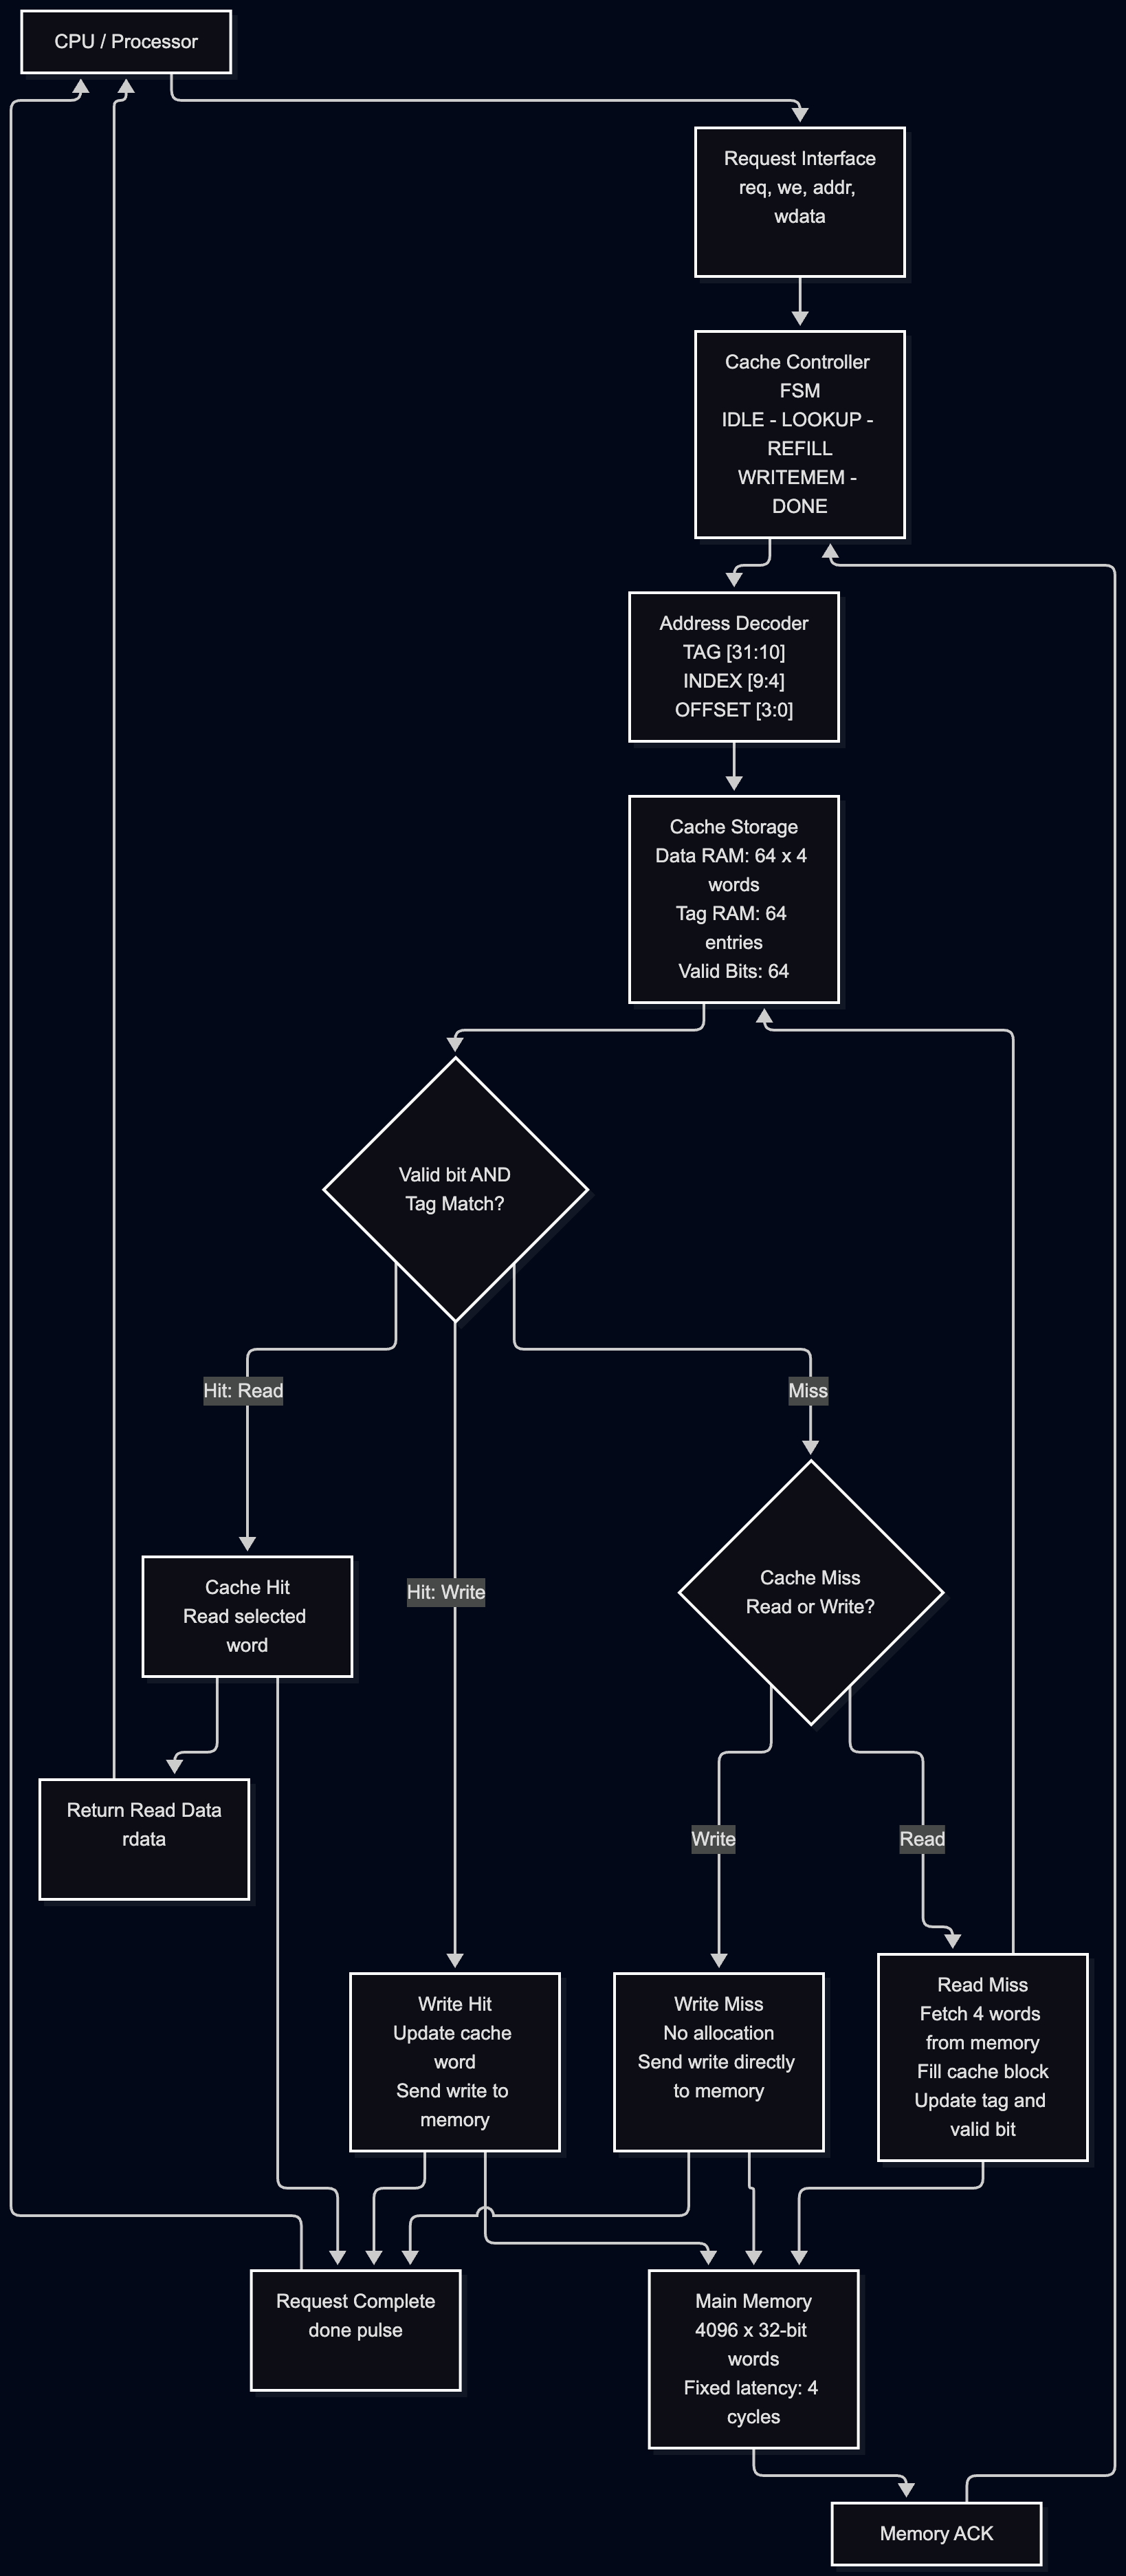
\includegraphics[width=\columnwidth]{figures/block_diagram.png}
\caption{Architectural block diagram of the direct-mapped cache controller interfacing the processor request interface with main memory.}
\label{fig:block_diagram}
\end{figure}

The architecture utilizes a 32-bit byte address decomposed deterministically according to parameter specifications:
\begin{itemize}
    \item \textbf{Byte and Word Offset} ($\text{addr}[3:0]$): The 4-bit offset field comprises bits $[1:0]$ for byte selection within a 32-bit word and bits $[3:2]$ ($\text{word}$) to index one of the four words in the block.
    \item \textbf{Index Field} ($\text{addr}[9:4]$): The 6-bit index field ($\text{INDEX\_BITS}=6$) addresses one of the $2^6 = 64$ lines in the direct-mapped array.
    \item \textbf{Tag Field} ($\text{addr}[31:10]$): The remaining 22 bits constitute the tag field, which uniquely identifies the memory block residing in the indexed cache line.
\end{itemize}

Physical storage within the controller consists of three dedicated structures:
\begin{enumerate}
    \item \textbf{Data RAM}: An array of $64 \times 4 = 256$ 32-bit words (8,192 bits total), indexed jointly by $\{\text{idx}, \text{word}\}$.
    \item \textbf{Tag RAM}: An array of 64 entries of 22 bits each (1,408 bits total), indexed by $\text{idx}$.
    \item \textbf{Valid RAM}: A 64-bit register vector ($\text{valid\_ram}[63:0]$) cleared to zero during synchronous reset.
\end{enumerate}

\subsection{Finite State Machine (FSM) Operation}
The controller coordinates memory transactions and processor handshakes through an explicit 5-state FSM: \texttt{IDLE} (0), \texttt{LOOKUP} (1), \texttt{REFILL} (2), \texttt{WRITEMEM} (3), and \texttt{DONE} (4), depicted in Fig.~\ref{fig:fsm}. The output signal \texttt{busy} remains asserted ($\text{busy} = (\text{state} \neq \text{IDLE})$) throughout transaction processing, deasserting when returning to \texttt{IDLE}.

\begin{figure}[htbp]
\centering
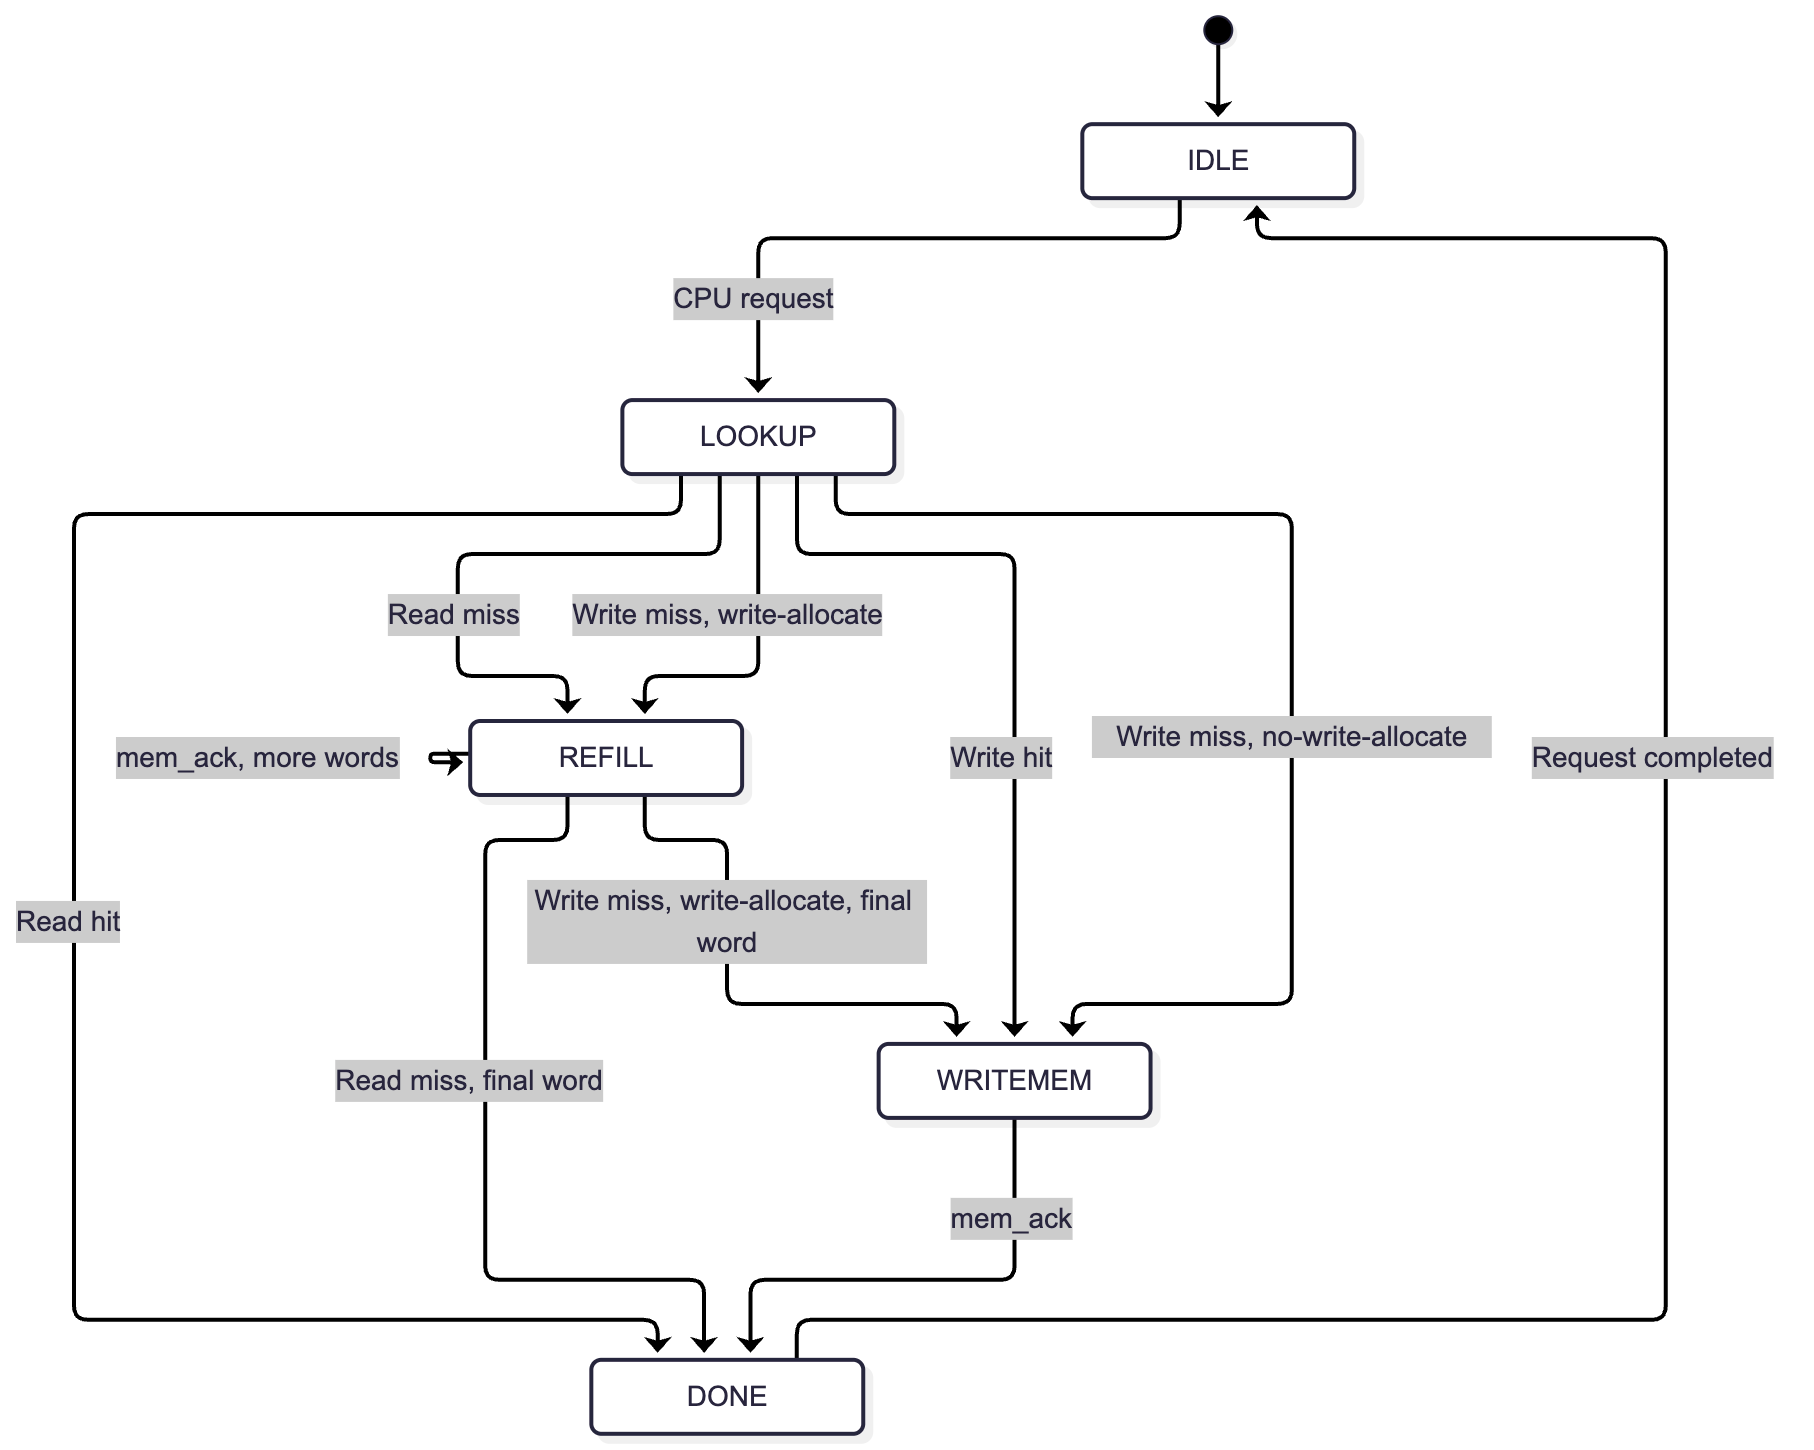
\includegraphics[width=0.85\columnwidth]{figures/fsm_diagram.png}
\caption{Finite State Machine (FSM) state transition diagram for cache request handling, memory refill, and write-through operations.}
\label{fig:fsm}
\end{figure}

The operational states execute as follows:
\begin{enumerate}
    \item \textbf{IDLE}: The controller awaits a CPU request. Upon assertion of \texttt{req}, the controller latches address (\texttt{l\_addr}), write data (\texttt{l\_wdata}), and write-enable (\texttt{l\_we}), transitioning to \texttt{LOOKUP}.
    \item \textbf{LOOKUP}: Hit evaluation occurs combinationally:
    \begin{equation}
        \text{hit} = \text{valid\_ram}[\text{idx}] \land (\text{tag\_ram}[\text{idx}] == \text{tag})
    \end{equation}
    If a hit occurs on a read operation ($\text{l\_we}=0$), the statistics counter \texttt{hits} increments, read data is driven combinationally from $\text{data\_ram}[\{\text{idx}, \text{word}\}]$, and the FSM transitions directly to \texttt{DONE}. If a hit occurs on a write operation ($\text{l\_we}=1$), \texttt{data\_ram} is updated immediately, write-through signals are asserted ($\text{mem\_req}=1, \text{mem\_we}=1, \text{mem\_addr}=\text{l\_addr}[31:2]$), and the FSM transitions to \texttt{WRITEMEM}.
    
    If a miss occurs, \texttt{misses} increments. On a read miss, the FSM transitions to \texttt{REFILL} to fetch the four-word line from main memory. On a write miss, state progression depends strictly upon the parameter \texttt{WRITE\_ALLOCATE}: under default no-write-allocate ($\text{WRITE\_ALLOCATE}=0$), the write bypasses cache allocation, posting directly to memory via \texttt{WRITEMEM}; under write-allocate ($\text{WRITE\_ALLOCATE}=1$), the FSM initiates a block refill via \texttt{REFILL} prior to completing the write.
    \item \textbf{REFILL}: The controller retrieves four words sequentially from memory. For each asserted \texttt{mem\_ack}, \texttt{mem\_reads} increments and the incoming word is written to $\text{data\_ram}[\{\text{idx}, \text{cnt}\}]$. Upon receipt of the fourth word ($\text{cnt}=3$), $\text{valid\_ram}[\text{idx}]$ is set, $\text{tag\_ram}[\text{idx}]$ is updated with the latched tag, and the line allocation completes. If the refill was triggered by a write miss with write-allocate ($\text{pending\_write}=1$), the pending write data is written to cache, and the write-through transaction is issued to \texttt{WRITEMEM}; otherwise, the FSM advances to \texttt{DONE}.
    \item \textbf{WRITEMEM}: The controller maintains memory write request lines until main memory responds with \texttt{mem\_ack}. Upon acknowledgment, \texttt{mem\_writes} increments, write lines deassert, and the FSM advances to \texttt{DONE}.
    \item \textbf{DONE}: The controller asserts a single-cycle completion pulse (\texttt{done}) to notify the CPU that data is valid or the write is complete, transitioning unconditionally to \texttt{IDLE}.
\end{enumerate}

\subsection{Memory Interface and Write Policy}
The memory interface implements an explicit synchronous request-acknowledgment handshake. Main memory is word-addressed (\texttt{mem\_addr} represents word indices $\text{addr}[31:2]$). The memory model (\texttt{main\_mem.v}) simulates access latency via parameter \texttt{LAT}, delaying \texttt{mem\_ack} assertion by exactly \texttt{LAT} clock cycles per access.

The cache implements a write-through policy: all write operations propagate to main memory to guarantee coherence with backing storage. By default, the write-miss policy is \textbf{no-write-allocate} ($\text{WRITE\_ALLOCATE}=0$), in which write misses update backing store without evicting resident cache blocks. Setting $\text{WRITE\_ALLOCATE}=1$ enables \textbf{write-allocate}, bringing the missing block into cache on write misses.

\section{Results and Discussion}
All reported performance and hardware metrics originate directly from simulation logs, testbench execution outputs, and synthesis reports preserved in the repository.

\subsection{Hit and Miss Rates}
Workload evaluation was conducted using eight standardized memory access traces running against the 1~KB / 16-byte block / $\text{LAT}=4$ baseline configuration in \texttt{tb\_trace.v}. Table~\ref{tab:hit_miss} details the measured counts and percentages, and Fig.~\ref{fig:hit_miss} illustrates the comparison.

% Source: docs/results/results_table.csv, line 1
\begin{table}[htbp]
\caption{Cache Hit and Miss Rates across Workload Traces (1~KB, 16~B Block, $\text{LAT}=4$)}
\label{tab:hit_miss}
\centering
\begin{tabular}{lrrrrr}
\toprule
\textbf{Trace} & \textbf{Accesses} & \textbf{Hits} & \textbf{Misses} & \textbf{Hit Rate} & \textbf{Miss Rate} \\
\midrule
% Source: docs/results/results_table.csv, line 2
sequential & 512 & 384 & 128 & 75.00\% & 25.00\% \\
% Source: docs/results/results_table.csv, line 3
random & 2000 & 479 & 1521 & 23.95\% & 76.05\% \\
% Source: docs/results/results_table.csv, line 4
repeated & 800 & 796 & 4 & 99.50\% & 0.50\% \\
% Source: docs/results/results_table.csv, line 5
stride16 & 1000 & 0 & 1000 & 0.00\% & 100.00\% \\
% Source: docs/results/results_table.csv, line 6
stride1024 & 1000 & 0 & 1000 & 0.00\% & 100.00\% \\
% Source: docs/results/results_table.csv, line 7
matrix\_rowmajor & 1024 & 768 & 256 & 75.00\% & 25.00\% \\
% Source: docs/results/results_table.csv, line 8
matrix\_colmajor & 1024 & 0 & 1024 & 0.00\% & 100.00\% \\
% Source: docs/results/results_table.csv, line 9
writes & 38 & 27 & 11 & 71.05\% & 28.95\% \\
\bottomrule
\end{tabular}
\end{table}

\begin{figure}[htbp]
\centering
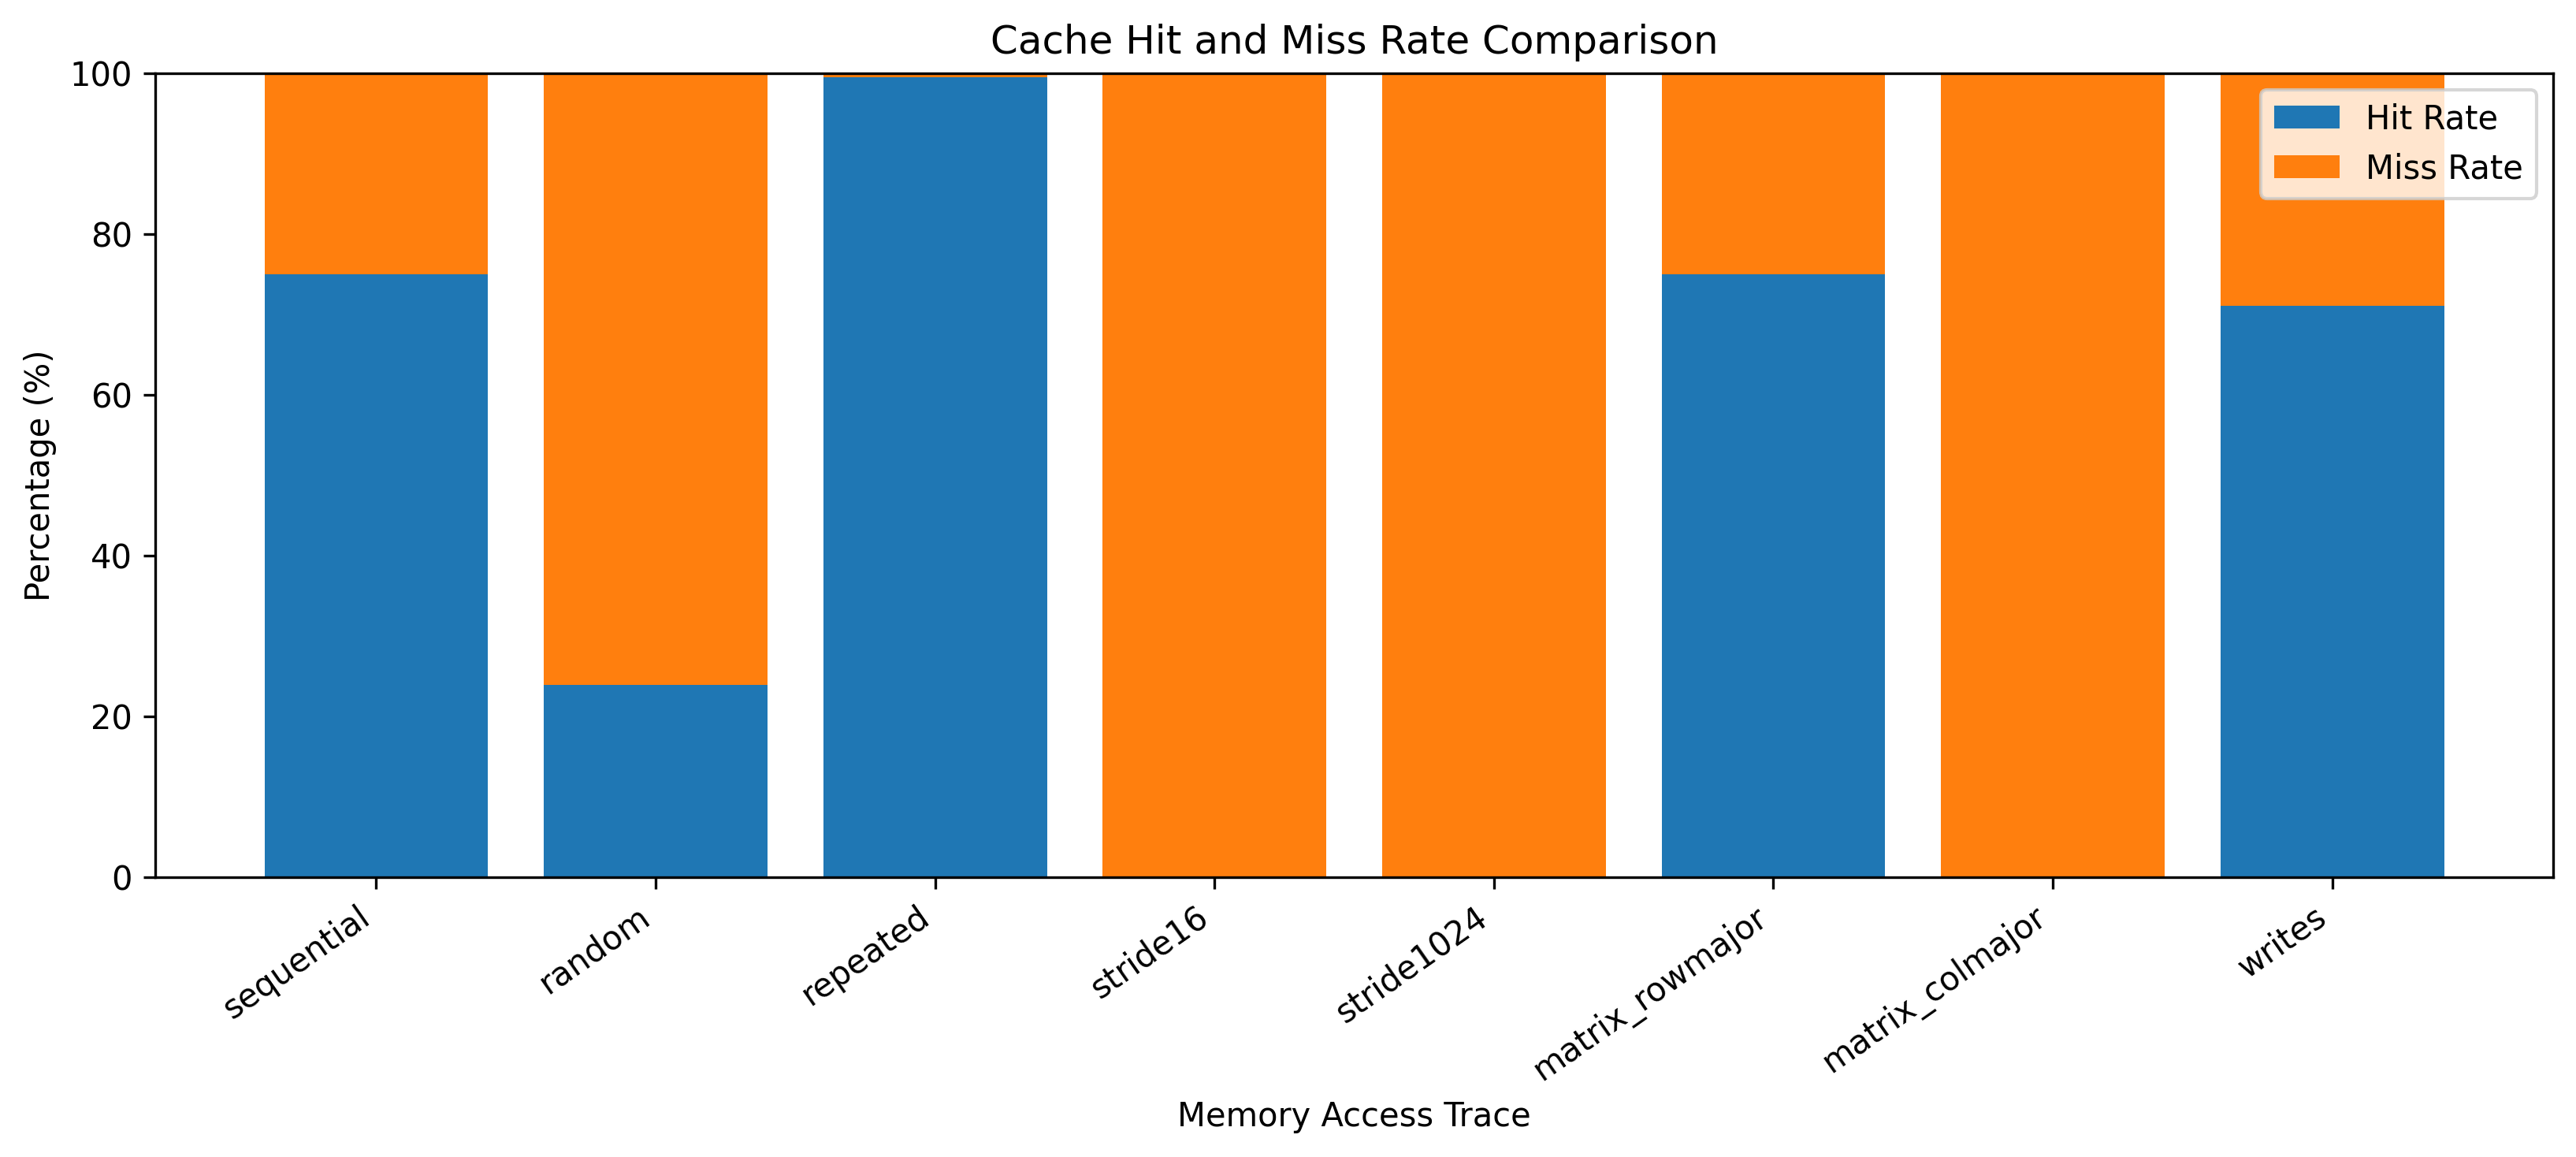
\includegraphics[width=\columnwidth]{figures/hit_miss_comparison.png}
\caption{Cache hit and miss counts across the eight evaluation traces on the baseline 1~KB direct-mapped cache.}
\label{fig:hit_miss}
\end{figure}

Sequential and matrix row-major traces demonstrate the efficacy of spatial locality: each compulsory miss fetches four consecutive words, satisfying the subsequent three accesses directly from cache ($3/4 = 75.00\%$ hit rate). The repeated trace exploits temporal locality, achieving 99.50\% hit rate because its 16-word working set fits entirely within cache lines. Conversely, stride-16 touches only one word per block, producing 0.00\% hits. Stride-1024 and matrix column-major exhibit pathological index collisions (addresses differing by multiples of 1~KB map to identical cache lines), yielding 0.00\% hits due to continuous conflict thrashing. 

For the random workload over a 4~KB address space, 479 hits out of 2,000 accesses yield an exact hit rate of $23.95\%$ and a miss rate of $76.05\%$. These values round to $24.0\%$ and $76.0\%$ at one decimal place, corresponding to the $23.9\%$ and $76.0\%$ figures recorded in raw integer-truncated script logs. The hit rate reflects the ratio of cache capacity (1~KB) to the active 4~KB address footprint.

\textit{Takeaway:} Cache hit rates range from 0.00\% to 99.50\%, dictated entirely by whether memory access patterns exhibit spatial alignment or suffer from direct-mapped conflict thrashing.

\subsection{Average Memory Access Time (AMAT)}
AMAT quantifies memory hierarchy performance and is calculated using:
\begin{equation}
    \text{AMAT} = \text{Hit Time} + (\text{Miss Rate} \times \text{Miss Penalty})
\end{equation}
In the simulated architecture with $\text{LAT}=4$, timing measurements establish:
\begin{itemize}
    \item \textbf{Hit Time}: 3 clock cycles (\texttt{IDLE} $\rightarrow$ \texttt{LOOKUP} $\rightarrow$ \texttt{DONE} $\rightarrow$ \texttt{IDLE}).
    \item \textbf{Miss Penalty}: 20 clock cycles. A read miss refills 4 words, each requiring $\text{LAT}+1 = 5$ cycles (4 latency cycles plus 1 handshake cycle), totaling $4 \times 5 = 20$ cycles. Total miss latency is $3 + 20 = 23$ cycles.
\end{itemize}
Substituting these verified parameters yields the baseline evaluation formula:
\begin{equation}
    \text{AMAT} = 3 + (\text{Miss Rate} \times 20)
\end{equation}
For sequential access ($\text{Miss Rate} = 0.25$): $\text{AMAT} = 3 + (0.25 \times 20) = 8.00$ cycles, matching cycle-accurate simulation. For repeated access ($\text{Miss Rate} = 0.005$): $\text{AMAT} = 3 + (0.005 \times 20) = 3.10$ cycles.

It is critical to distinguish theoretical read AMAT from measured write latency. The standard formula assumes read-dominant access where a miss incurs a full 20-cycle block refill. For the write workload (\texttt{writes.trace}: 20 reads, 18 writes, $28.95\%$ miss rate), applying the read AMAT equation would yield $3 + (0.2895 \times 20) = 8.79$ cycles. However, cycle-accurate simulation in \texttt{tb\_trace.v} measures an average access latency of exactly \textbf{8.53 clock cycles}.

This exact measurement is traceable directly to the cycle accumulation in \texttt{tb\_trace.v} (accumulating 324 cycles over 38 accesses): (1) 6 read misses $\times 23\text{ cycles} = 138$; (2) 14 read hits $\times 3\text{ cycles} = 42$; (3) 13 write hits $\times 8\text{ cycles} = 104$; and (4) 5 write misses $\times 8\text{ cycles} = 40$. Summing these components yields:
\begin{equation}
    \text{Cycles}_{\text{total}} = 138 + 42 + 104 + 40 = 324\text{ cycles}
\end{equation}
\begin{equation}
    \text{Avg Latency} = \frac{324\text{ cycles}}{38\text{ accesses}} = 8.5263 \approx 8.53\text{ cycles}
\end{equation}
Under the default no-write-allocate policy, write misses do not refill a 4-word block; instead, they post a single word directly to memory via \texttt{WRITEMEM}, completing in only 8 cycles ($3\text{ lookup} + \text{LAT memory write} + 1\text{ handshake} = 8$). Consequently, the measured 8.53-cycle latency accurately accounts for write-through execution paths, as confirmed by the simulation output log:
\begin{quote}
\small\texttt{Trace: writes.trace | accesses=38 hits=27 misses=11}\\
\small\texttt{hit\_rate=71.1\% miss\_rate=28.9\%}\\
\small\texttt{avg\_cycles\_per\_access=8.53 AMAT(formula)=8.79}\\
\small\texttt{DATA CHECK PASSED}
\end{quote}
Fig.~\ref{fig:amat} illustrates AMAT across traces.

\begin{figure}[htbp]
\centering
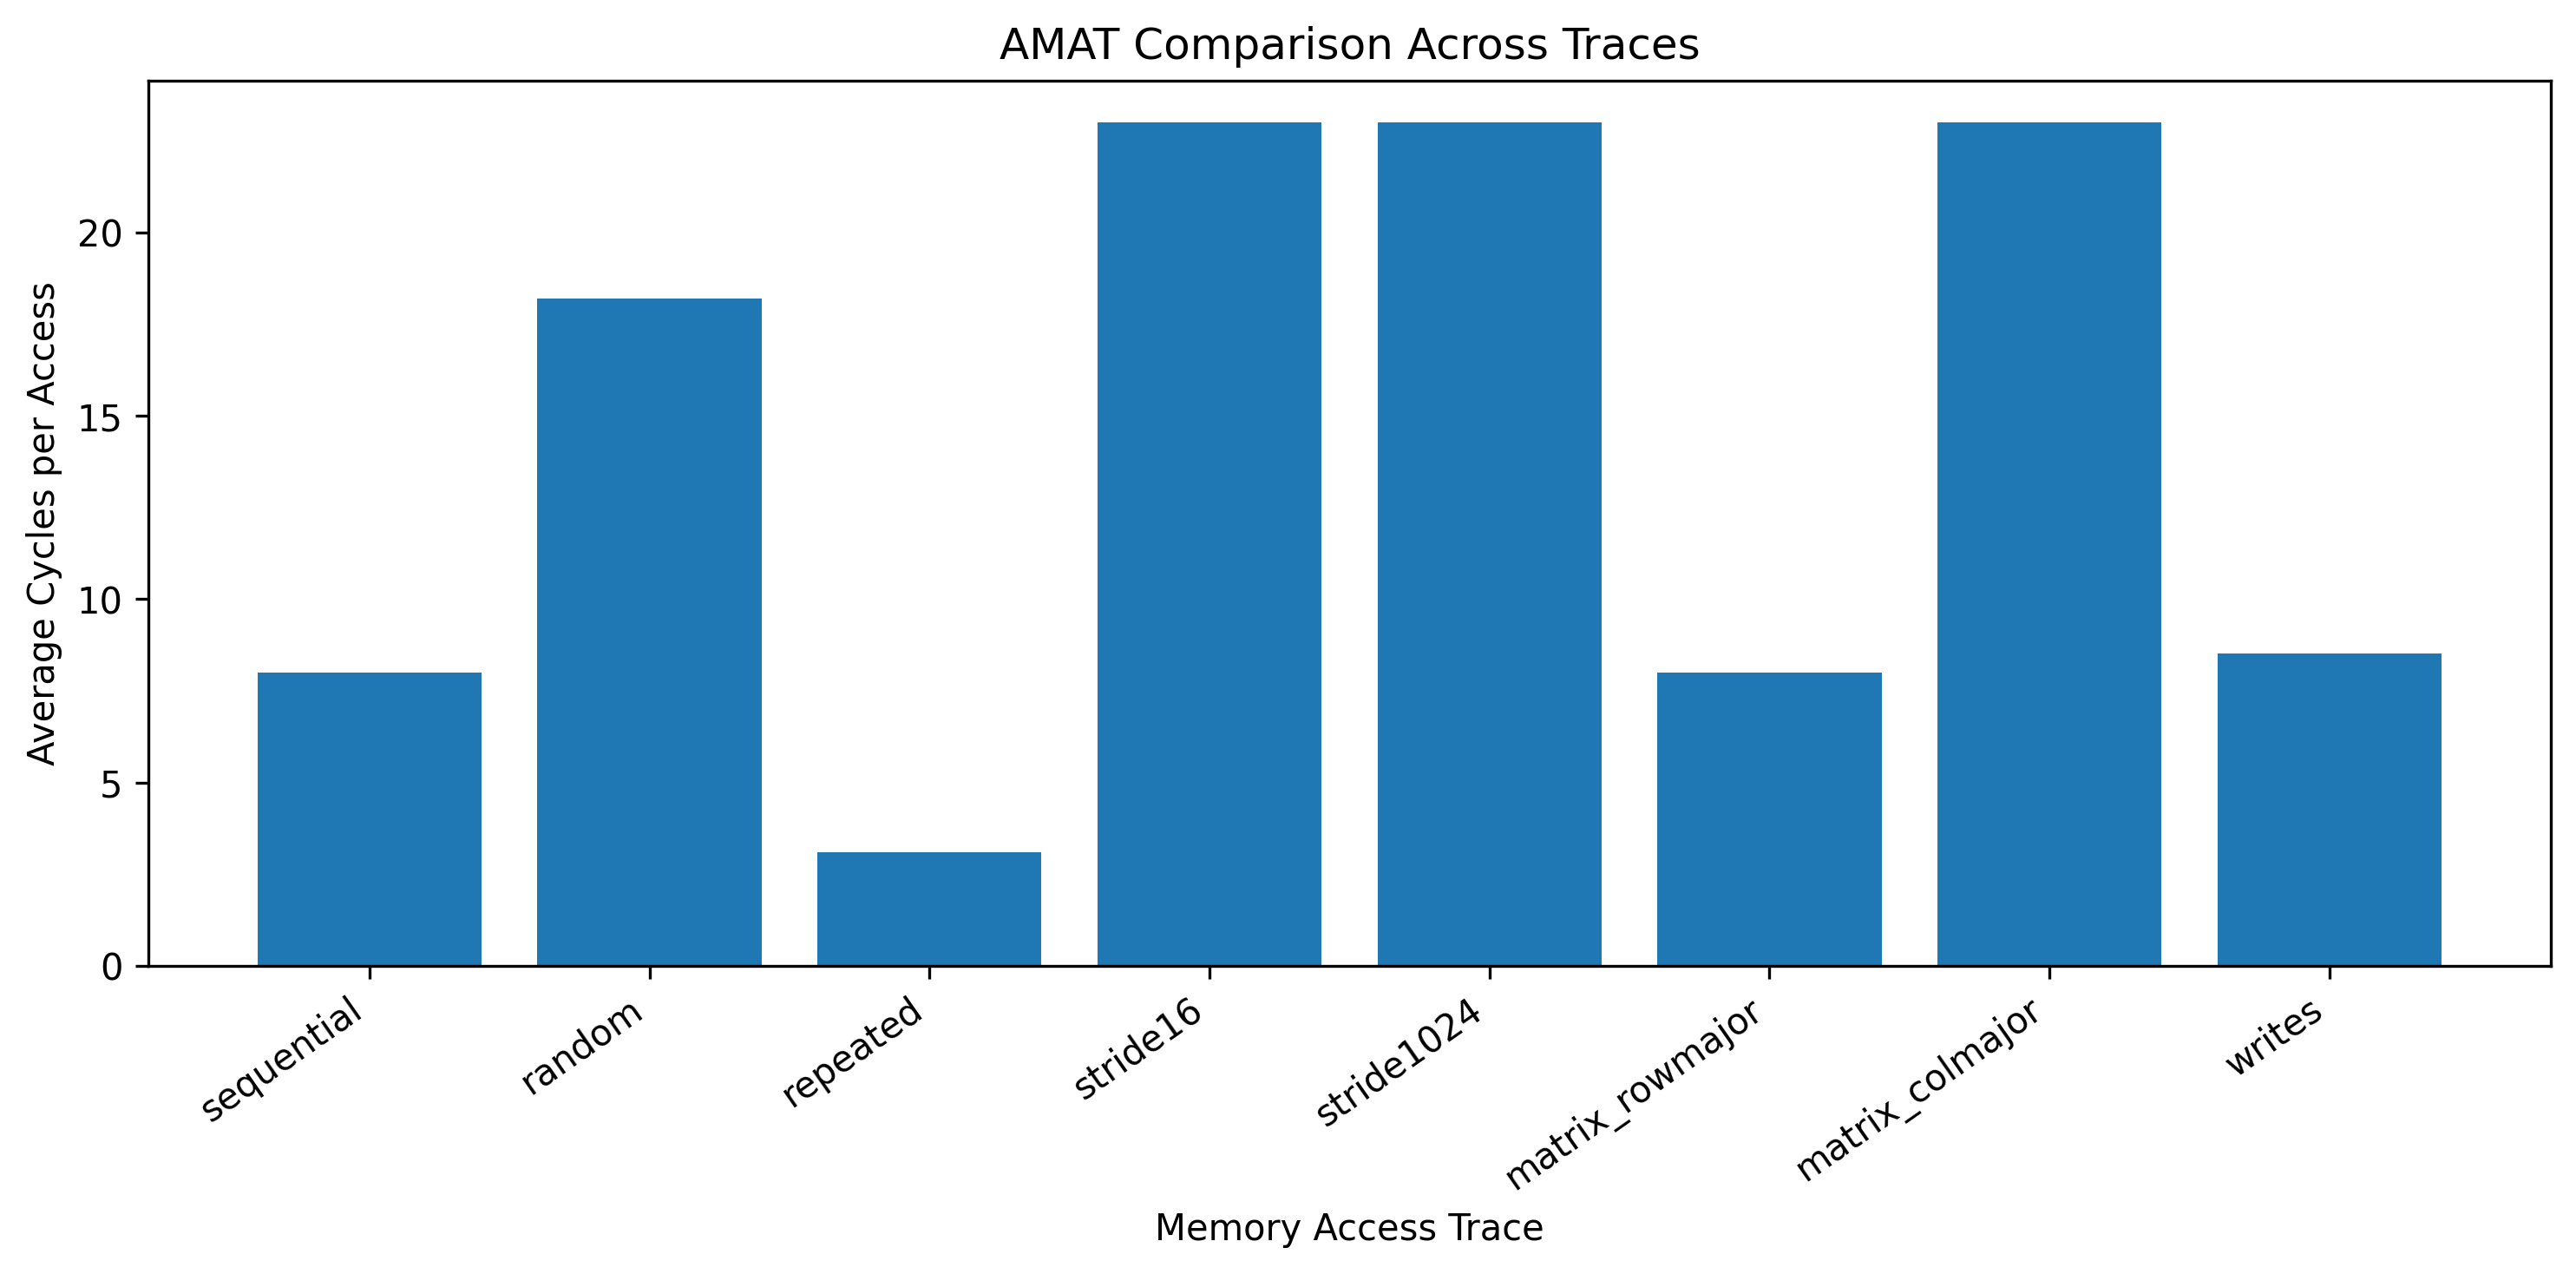
\includegraphics[width=\columnwidth]{figures/amat_comparison.png}
\caption{Average Memory Access Time (AMAT) in clock cycles across benchmark workloads (LAT = 4).}
\label{fig:amat}
\end{figure}

\textit{Takeaway:} AMAT scales linearly with read miss penalty (20 cycles at $\text{LAT}=4$), while write-containing workloads require measured cycle accounting due to single-word write-through timing.

\subsection{Cache versus No-Cache Comparison}
In a system without cache, the processor accesses main memory directly, incurring $\text{LAT}$ cycles per operation. Table~\ref{tab:nocache} evaluates average access cycles between the cache-enabled design and the no-cache baseline across memory latencies from $\text{LAT}=4$ to $\text{LAT}=100$.

% Source: docs/results/lat_sweep.csv, lines 1-6
\begin{table}[htbp]
\caption{Average Access Latency (Cycles): Cache vs. No-Cache Across Latencies}
\label{tab:nocache}
\centering
\begin{tabular}{lrrrr}
\toprule
\textbf{Trace} & \textbf{Config} & \textbf{LAT 4} & \textbf{LAT 20} & \textbf{LAT 100} \\
\midrule
% Source: docs/results/lat_sweep.csv, line 2
sequential & Cache / None & 8.00 / 4 & 24.00 / 20 & 104.00 / 100 \\
% Source: docs/results/lat_sweep.csv, line 3
random & Cache / None & 18.21 / 4 & 66.88 / 20 & 310.24 / 100 \\
% Source: docs/results/lat_sweep.csv, line 4
repeated & Cache / None & 3.10 / 4 & 3.42 / 20 & 5.02 / 100 \\
% Source: docs/results/lat_sweep.csv, line 5
matrix\_rowmajor & Cache / None & 8.00 / 4 & 24.00 / 20 & 104.00 / 100 \\
% Source: docs/results/lat_sweep.csv, line 6
matrix\_colmajor & Cache / None & 23.00 / 4 & 87.00 / 20 & 407.00 / 100 \\
\bottomrule
\end{tabular}
\end{table}

The empirical results reveal that caching is only advantageous when workload locality is high. On the repeated trace, the cache provides a dramatic advantage as memory latency grows, reducing access time from 100 cycles to 5.02 cycles at $\text{LAT}=100$ ($19.9\times$ speedup). However, on sequential and row-major workloads, the cache performs worse than no-cache across all latencies (e.g., 8.00 vs. 4 cycles at $\text{LAT}=4$, and 104.00 vs. 100 cycles at $\text{LAT}=100$). This occurs because the memory model lacks burst transfers: each refilled word pays the full $\text{LAT}$ cycles independently ($4 \times \text{LAT}$), negating the spatial locality benefit in raw cycle counts. For random and column-major patterns, fetching unreferenced words severely penalizes performance ($407.00$ vs. 100 cycles).

\textit{Takeaway:} Without memory burst modes, direct-mapped caching outperforms un-cached access only when temporal locality is exceptionally high, while low-locality workloads suffer substantial penalties from unamortized block refills.

\subsection{LAT Experiment --- LAT 2, 4, and 8}
The LAT sweep experiment across LAT values 2, 4, and 8 was conducted using the dedicated self-checking testbench \texttt{tb\_lat\_sweep.v}. Table~\ref{tab:lat_sweep_tb} presents the measured cycle latencies across six directed test phases.

% Source: docs/results/lat_2_4_8_sweep.csv, line 1
\begin{table}[htbp]
\caption{Measured Latencies from \texttt{tb\_lat\_sweep.v} across $\text{LAT}\in\{2, 4, 8\}$}
\label{tab:lat_sweep_tb}
\centering
\begin{tabular}{lrrr}
\toprule
\textbf{Directed Test Phase} & \textbf{LAT 2} & \textbf{LAT 4} & \textbf{LAT 8} \\
\midrule
% Source: docs/results/lat_2_4_8_sweep.csv, line 2
T1\_sequential (256 accesses) & 6.0 & 8.0 & 12.0 \\
% Source: docs/results/lat_2_4_8_sweep.csv, line 3
T2\_repeated (128 accesses) & 3.3 & 3.6 & 4.1 \\
% Source: docs/results/lat_2_4_8_sweep.csv, line 4
T3\_conflict (16 accesses) & 14.2 & 21.7 & 36.7 \\
% Source: docs/results/lat_2_4_8_sweep.csv, line 5
T4\_write\_policy (4 accesses) & 7.5 & 10.5 & 16.5 \\
% Source: docs/results/lat_2_4_8_sweep.csv, line 6
T5\_random (400 accesses) & 12.2 & 18.3 & 30.6 \\
% Source: docs/results/lat_2_4_8_sweep.csv, line 7
T6\_full\_line\_fill (64 accesses) & 15.0 & 23.0 & 39.0 \\
\bottomrule
\end{tabular}
\end{table}

In \texttt{tb\_lat\_sweep.v}, the T2 repeated test issues 128 accesses (8 loops of 16 words, lines 172--176). The first 16 words generate 4 compulsory misses, followed by 124 hits, producing a 96.88\% hit rate ($124/128$). The average access times scale gracefully from 3.3 cycles at $\text{LAT}=2$, to 3.6 cycles at $\text{LAT}=4$, and 4.1 cycles at $\text{LAT}=8$. Conversely, test T6 (full line fill, 64 compulsory misses) incurs full block refills on every access, scaling sharply from 15.0 cycles ($\text{LAT}=2$) to 23.0 cycles ($\text{LAT}=4$) and 39.0 cycles ($\text{LAT}=8$).

\textit{Takeaway:} Controlled parameter sweeping in \texttt{tb\_lat\_sweep.v} verifies that miss penalty scales as $4 \times (\text{LAT}+1)$, validating hardware refill timing across memory latency regimes.

\subsection{Latency Sweep}
The broader latency sweep evaluated system performance under memory latencies spanning two orders of magnitude: $\text{LAT}\in\{4, 10, 20, 50, 100\}$ using \texttt{tb\_trace.v}, charted in Fig.~\ref{fig:latency_sweep}. For repeated access, cycles per access increase minimally: 3.10 cycles at $\text{LAT}=4$, 3.22 at $\text{LAT}=10$, 3.42 at $\text{LAT}=20$, 4.02 at $\text{LAT}=50$, and 5.02 at $\text{LAT}=100$. Because miss rate is merely 0.50\%, 99.50\% of accesses complete in 3 cycles regardless of memory delay. Conversely, for matrix column-major (100\% miss rate), cycles per access equal $3 + 4 \times (\text{LAT}+1)$: 23.0 at $\text{LAT}=4$, 47.0 at $\text{LAT}=10$, 87.0 at $\text{LAT}=20$, 207.0 at $\text{LAT}=50$, and 407.0 at $\text{LAT}=100$.

\begin{figure}[htbp]
\centering
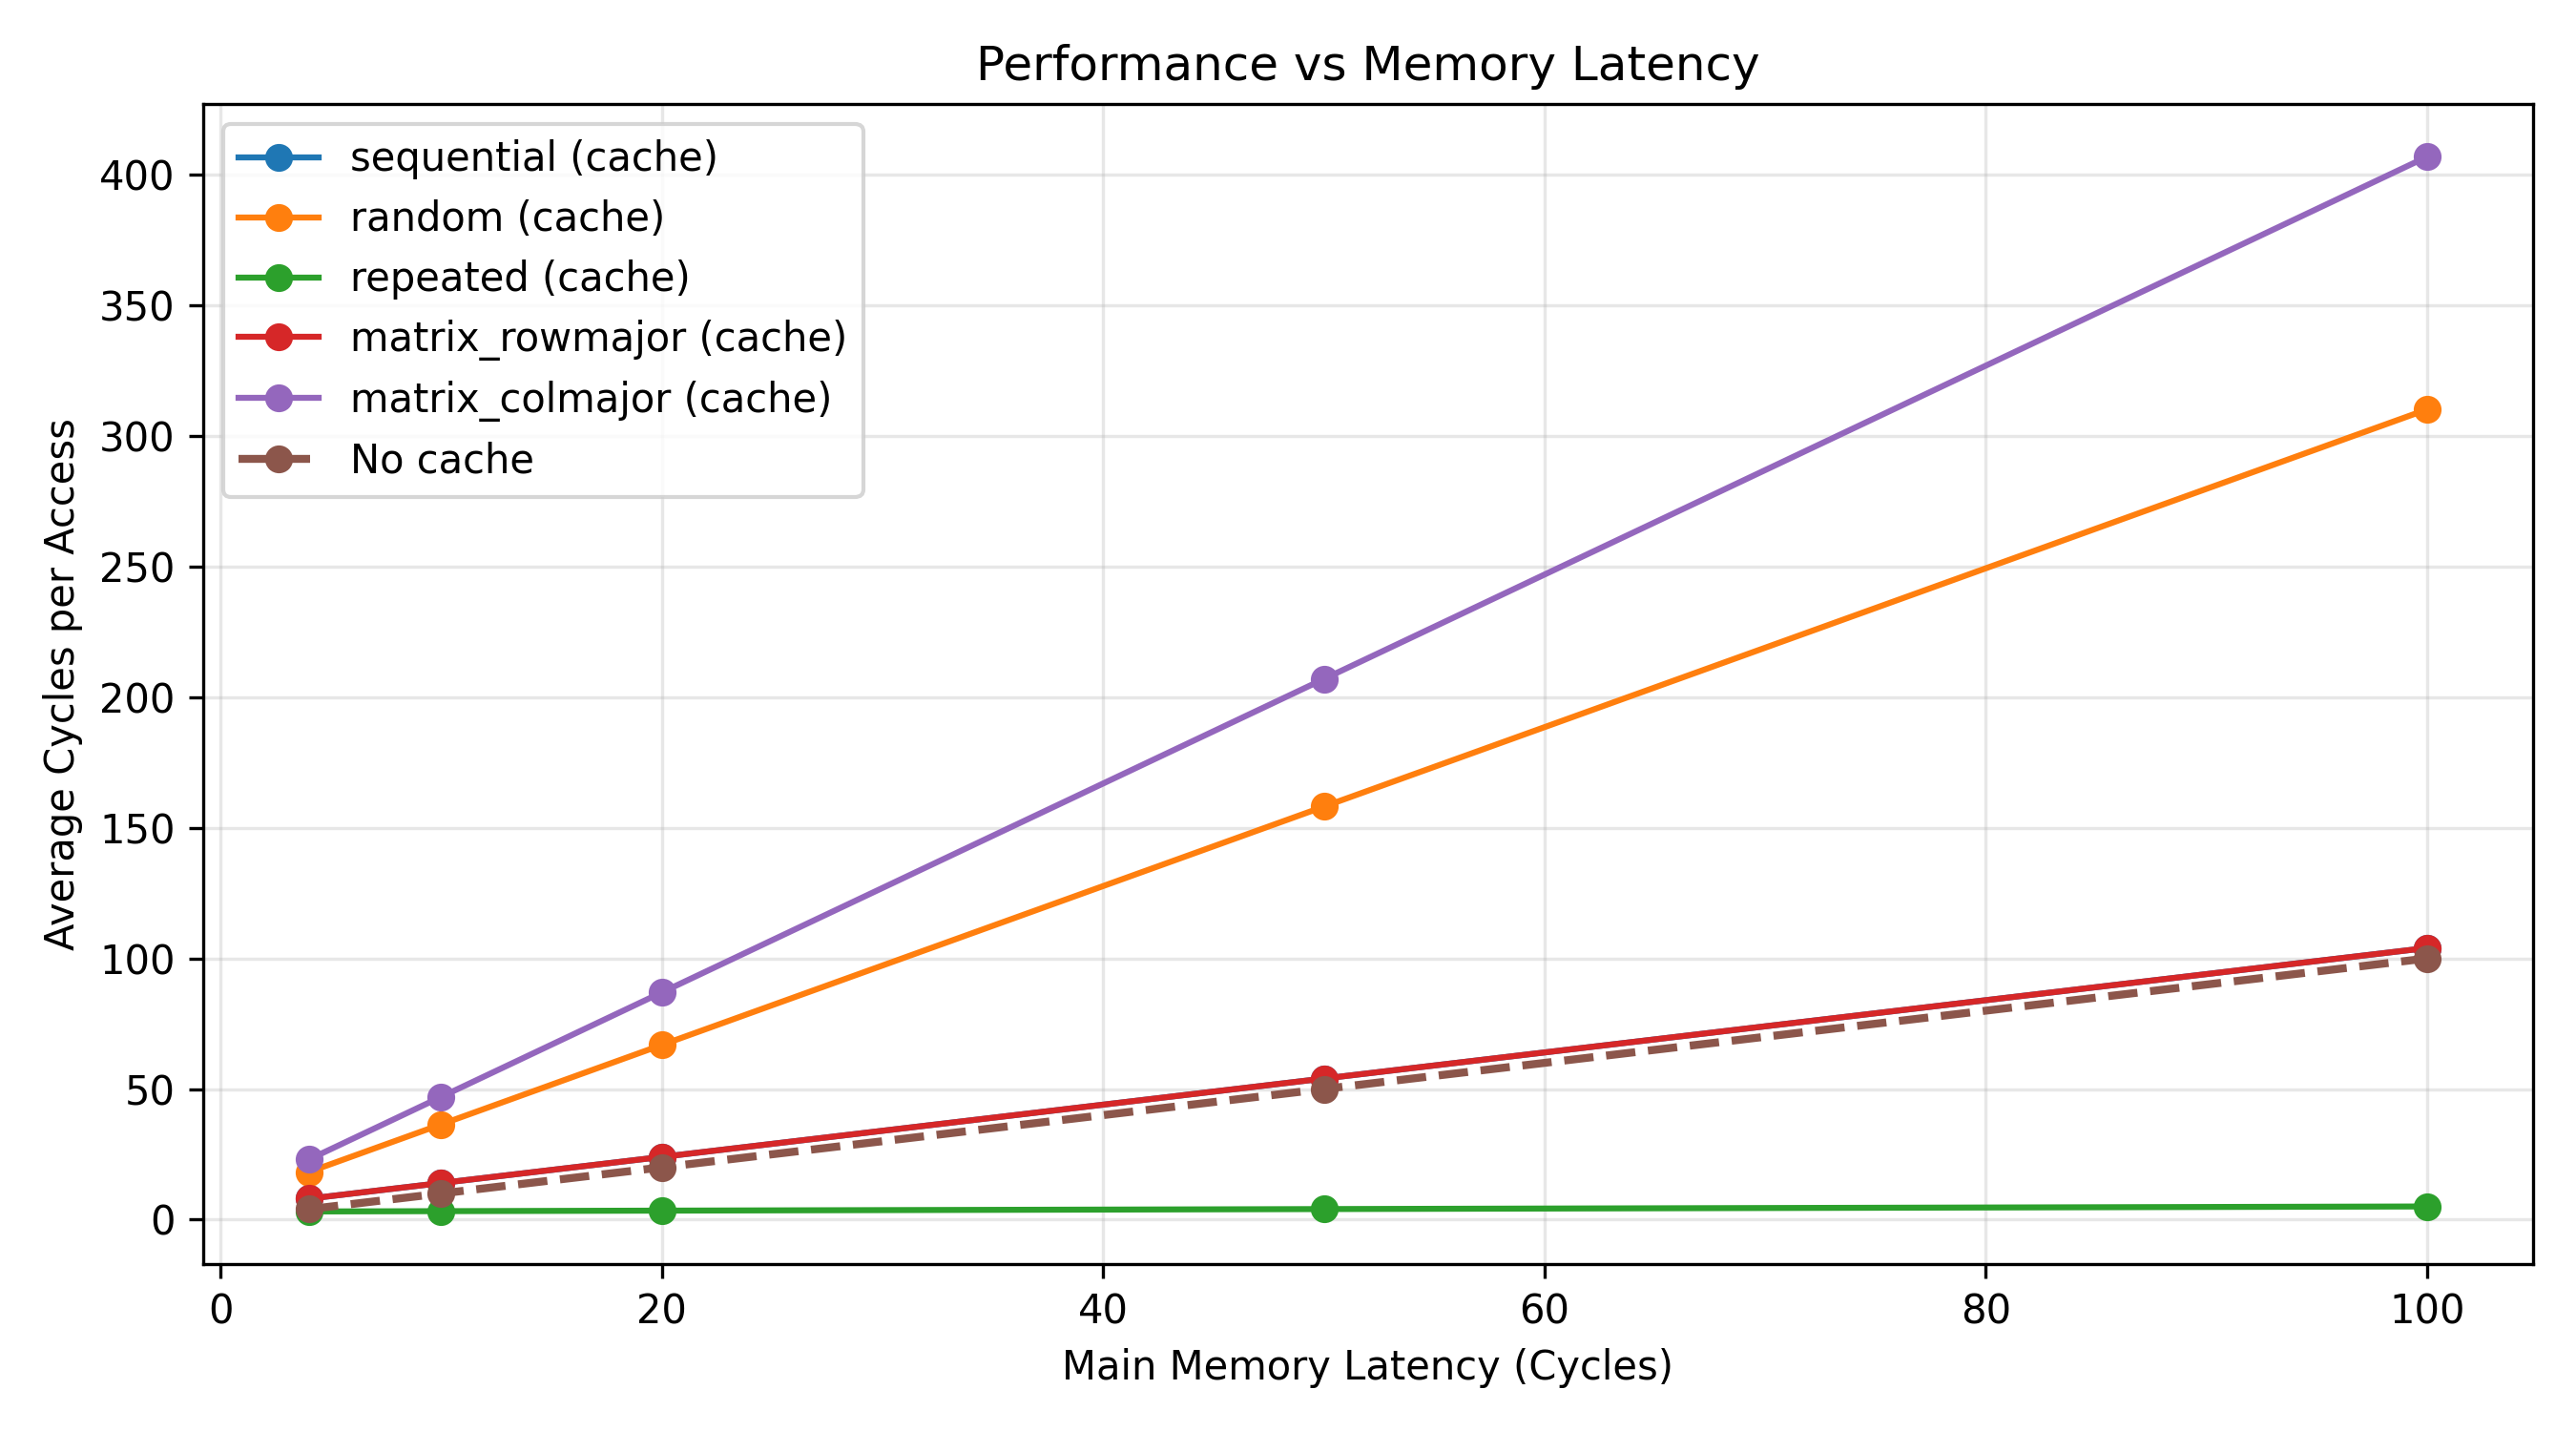
\includegraphics[width=\columnwidth]{figures/latency_sweep.png}
\caption{Latency sweep comparing access cycles across memory latency parameters from LAT = 4 to LAT = 100.}
\label{fig:latency_sweep}
\end{figure}

\textit{Takeaway:} High cache hit rates effectively decouple processor execution speed from backing memory latency, while low hit rates expose processor throughput directly to off-chip delays.

\subsection{Write-Policy Traffic Comparison}
The controller implements write-through caching, with no-write-allocate as the default policy and write-allocate selectable via \texttt{WRITE\_ALLOCATE}. Hardware counters \texttt{mem\_reads} and \texttt{mem\_writes} record the total 32-bit words transferred across the memory bus. Table~\ref{tab:traffic} summarizes comparative results from \texttt{tb\_traffic.v}, and Fig.~\ref{fig:traffic} depicts the traffic comparison.

% Source: docs/results/write_policy_traffic.csv, lines 1-19
\begin{table}[htbp]
\caption{Memory Traffic and Performance Comparison between Write Policies}
\label{tab:traffic}
\centering
\begin{tabular}{llrrrrr}
\toprule
\textbf{Trace} & \textbf{Policy} & \textbf{Hit Rate} & \textbf{Reads} & \textbf{Writes} & \textbf{Total} & \textbf{Avg Cyc} \\
\midrule
% Source: docs/results/write_policy_traffic.csv, line 9
writes & No-Alloc & 71.05\% & 24 & 18 & 42 & 8.53 \\
% Source: docs/results/write_policy_traffic.csv, line 18
writes & Allocate & 84.21\% & 24 & 18 & 42 & 8.53 \\
\midrule
% Source: docs/results/write_policy_traffic.csv, line 10
write\_stream & No-Alloc & 0.00\% & 0 & 512 & 512 & 8.00 \\
% Source: docs/results/write_policy_traffic.csv, line 19
write\_stream & Allocate & 75.00\% & 512 & 512 & 1024 & 13.00 \\
\bottomrule
\end{tabular}
\end{table}

\begin{figure}[htbp]
\centering
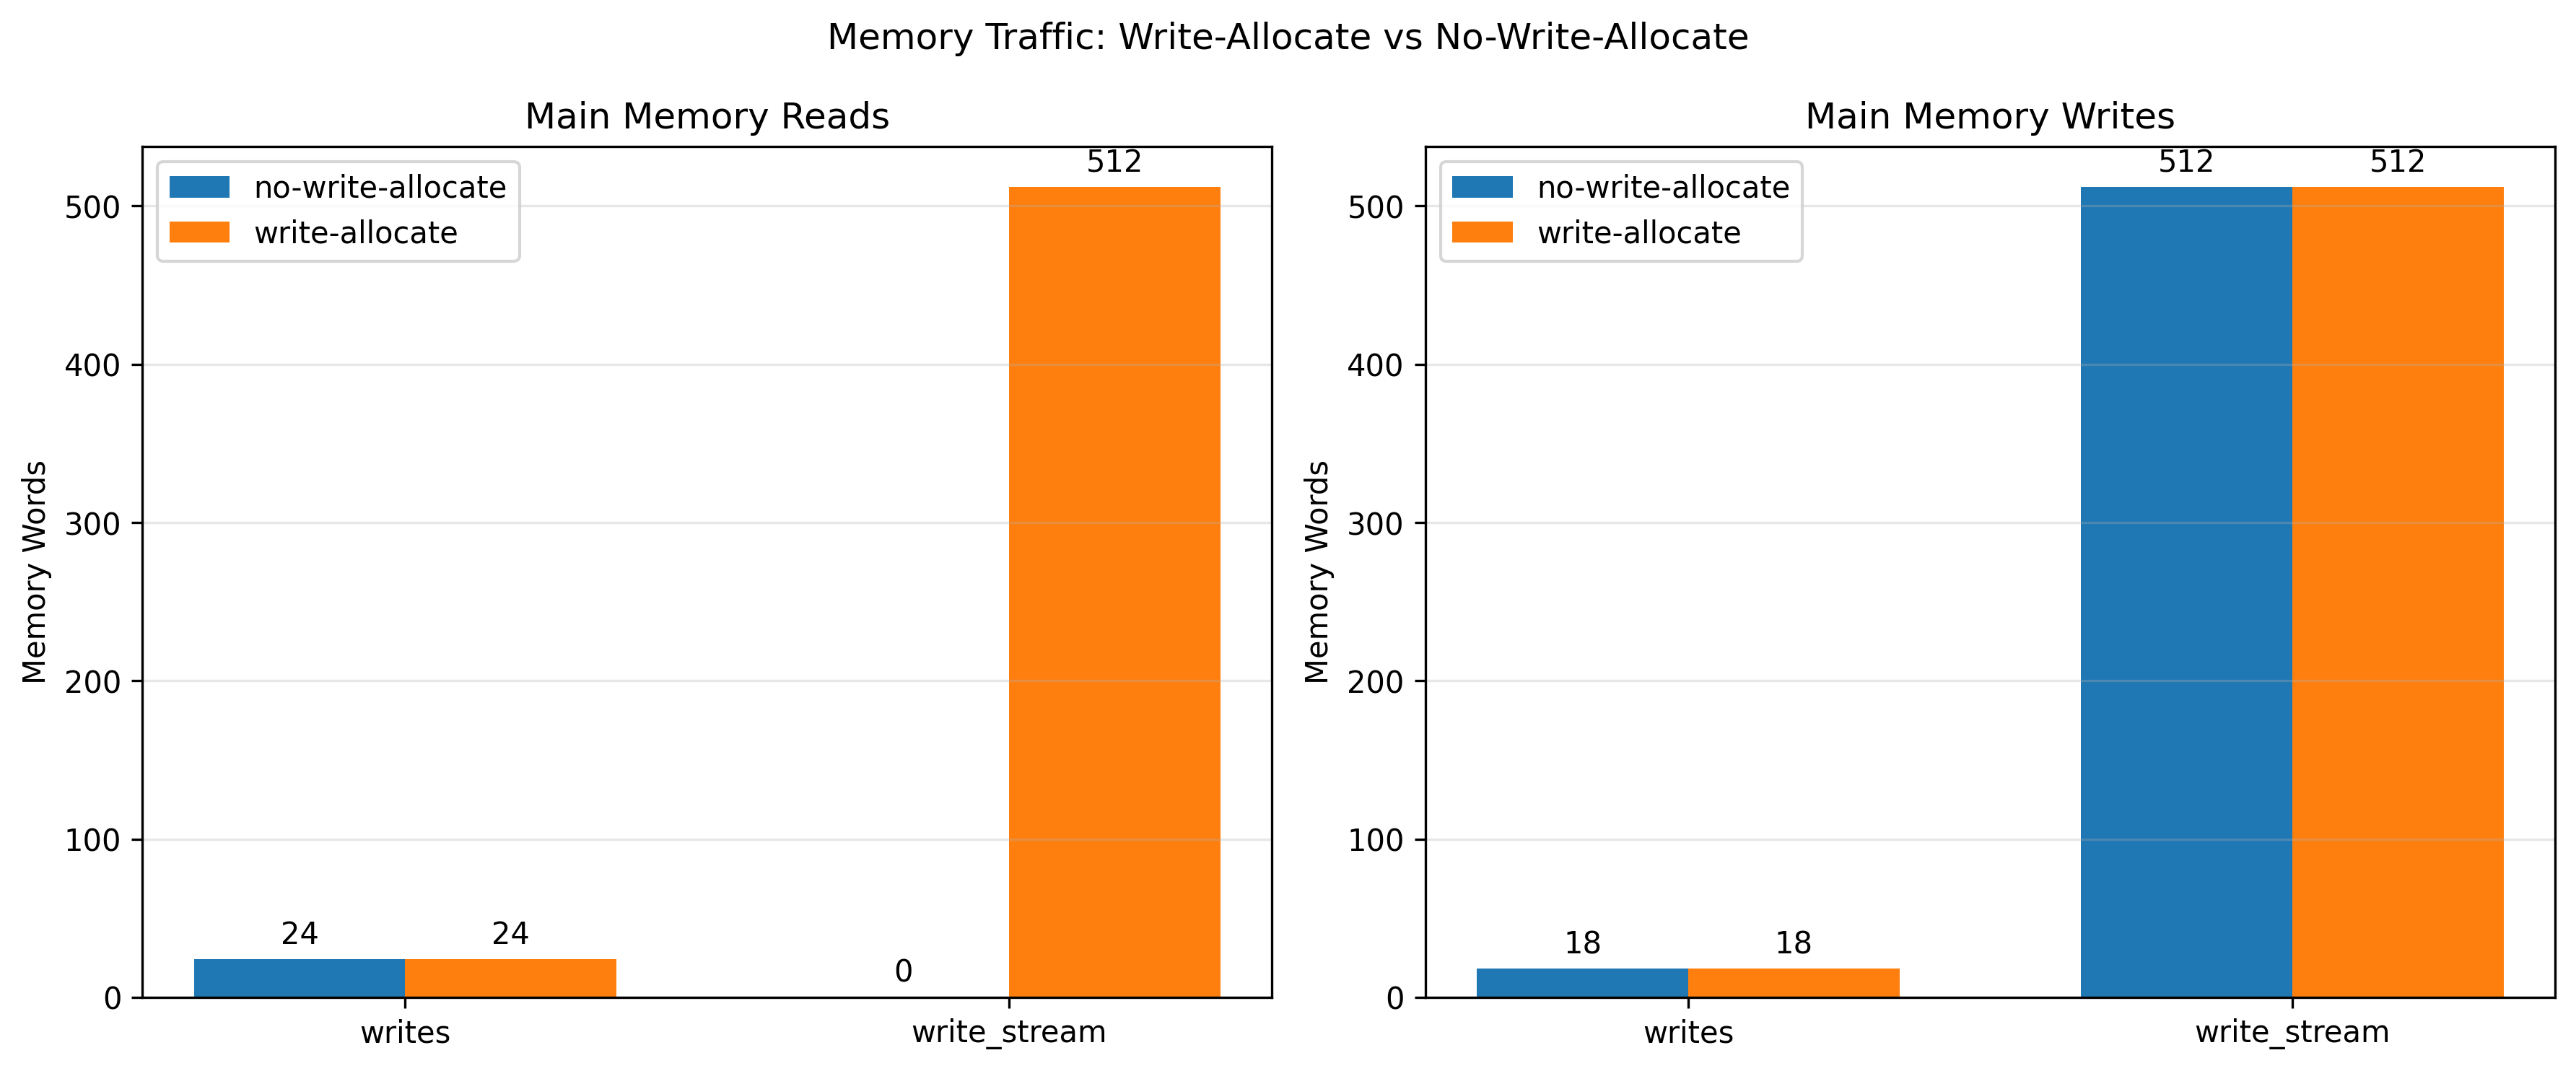
\includegraphics[width=\columnwidth]{figures/memory_traffic_comparison.png}
\caption{Memory traffic comparison (words transferred) between write-allocate and no-write-allocate policies on writes and write\_stream traces.}
\label{fig:traffic}
\end{figure}

For the eight read-only traces, both policies yield identical hit rates and traffic counts, confirming that \texttt{WRITE\_ALLOCATE} affects only the write-miss datapath. For \texttt{writes.trace} (20 reads, 18 writes with immediate read-back), write-allocate increases hit rate from 71.05\% to 84.21\% (hits increase from 27 to 32) with identical total memory traffic (42 words: 24 reads, 18 writes) and identical average latency (8.53 cycles). In contrast, on \texttt{write\_stream.trace} (512 sequential writes without subsequent reads), write-allocate incurs an unnecessary 4-word refill for every write miss, doubling memory traffic from 512 to 1024 words and increasing average cycle latency from 8.00 to 13.00 cycles.

\textit{Takeaway:} Write-allocate improves hit rate without traffic penalty when written lines experience subsequent read reuse, but doubles bus traffic and increases latency on write-once streaming workloads.

\subsection{Synthesis Results}
Physical implementation was conducted for the Lattice iCE40 HX8K FPGA (CT256 package) using the open-source Yosys (version 0.71) and nextpnr-ice40 (version 0.11.1) toolchain. Post-place-and-route results are presented in Table~\ref{tab:synthesis}, and resource utilization comparison is charted in Fig.~\ref{fig:synth_res}.

% Source: docs/synthesis/resource_utilization.csv, line 1
\begin{table}[htbp]
\caption{FPGA Synthesis and Timing Results on Lattice iCE40 HX8K}
\label{tab:synthesis}
\centering
\begin{tabular}{lrr}
\toprule
\textbf{Metric} & \textbf{1~KB Cache (64 lines)} & \textbf{512~B Cache (32 lines)} \\
\midrule
% Source: docs/synthesis/resource_utilization.csv, lines 2-3
Generic Cells & 30,922 & 15,652 \\
Generic Flip-Flops & 9,935 & 5,134 \\
LUT4 Cells & 491 & 412 \\
Carry Cells & 155 & 154 \\
Mapped Flip-Flops & 383 & 352 \\
Block RAMs (\texttt{SB\_RAM40\_4K}) & 4 / 32 (12\%) & 4 / 32 (12\%) \\
Placed Logic Cells & 740 / 7,680 (9\%) & 662 / 7,680 (8\%) \\
Critical Path Delay & 12.52~ns & 12.51~ns \\
Max Frequency ($F_{\max}$) & 79.85~MHz & 79.90~MHz \\
\bottomrule
\end{tabular}
\end{table}

\begin{figure}[htbp]
\centering
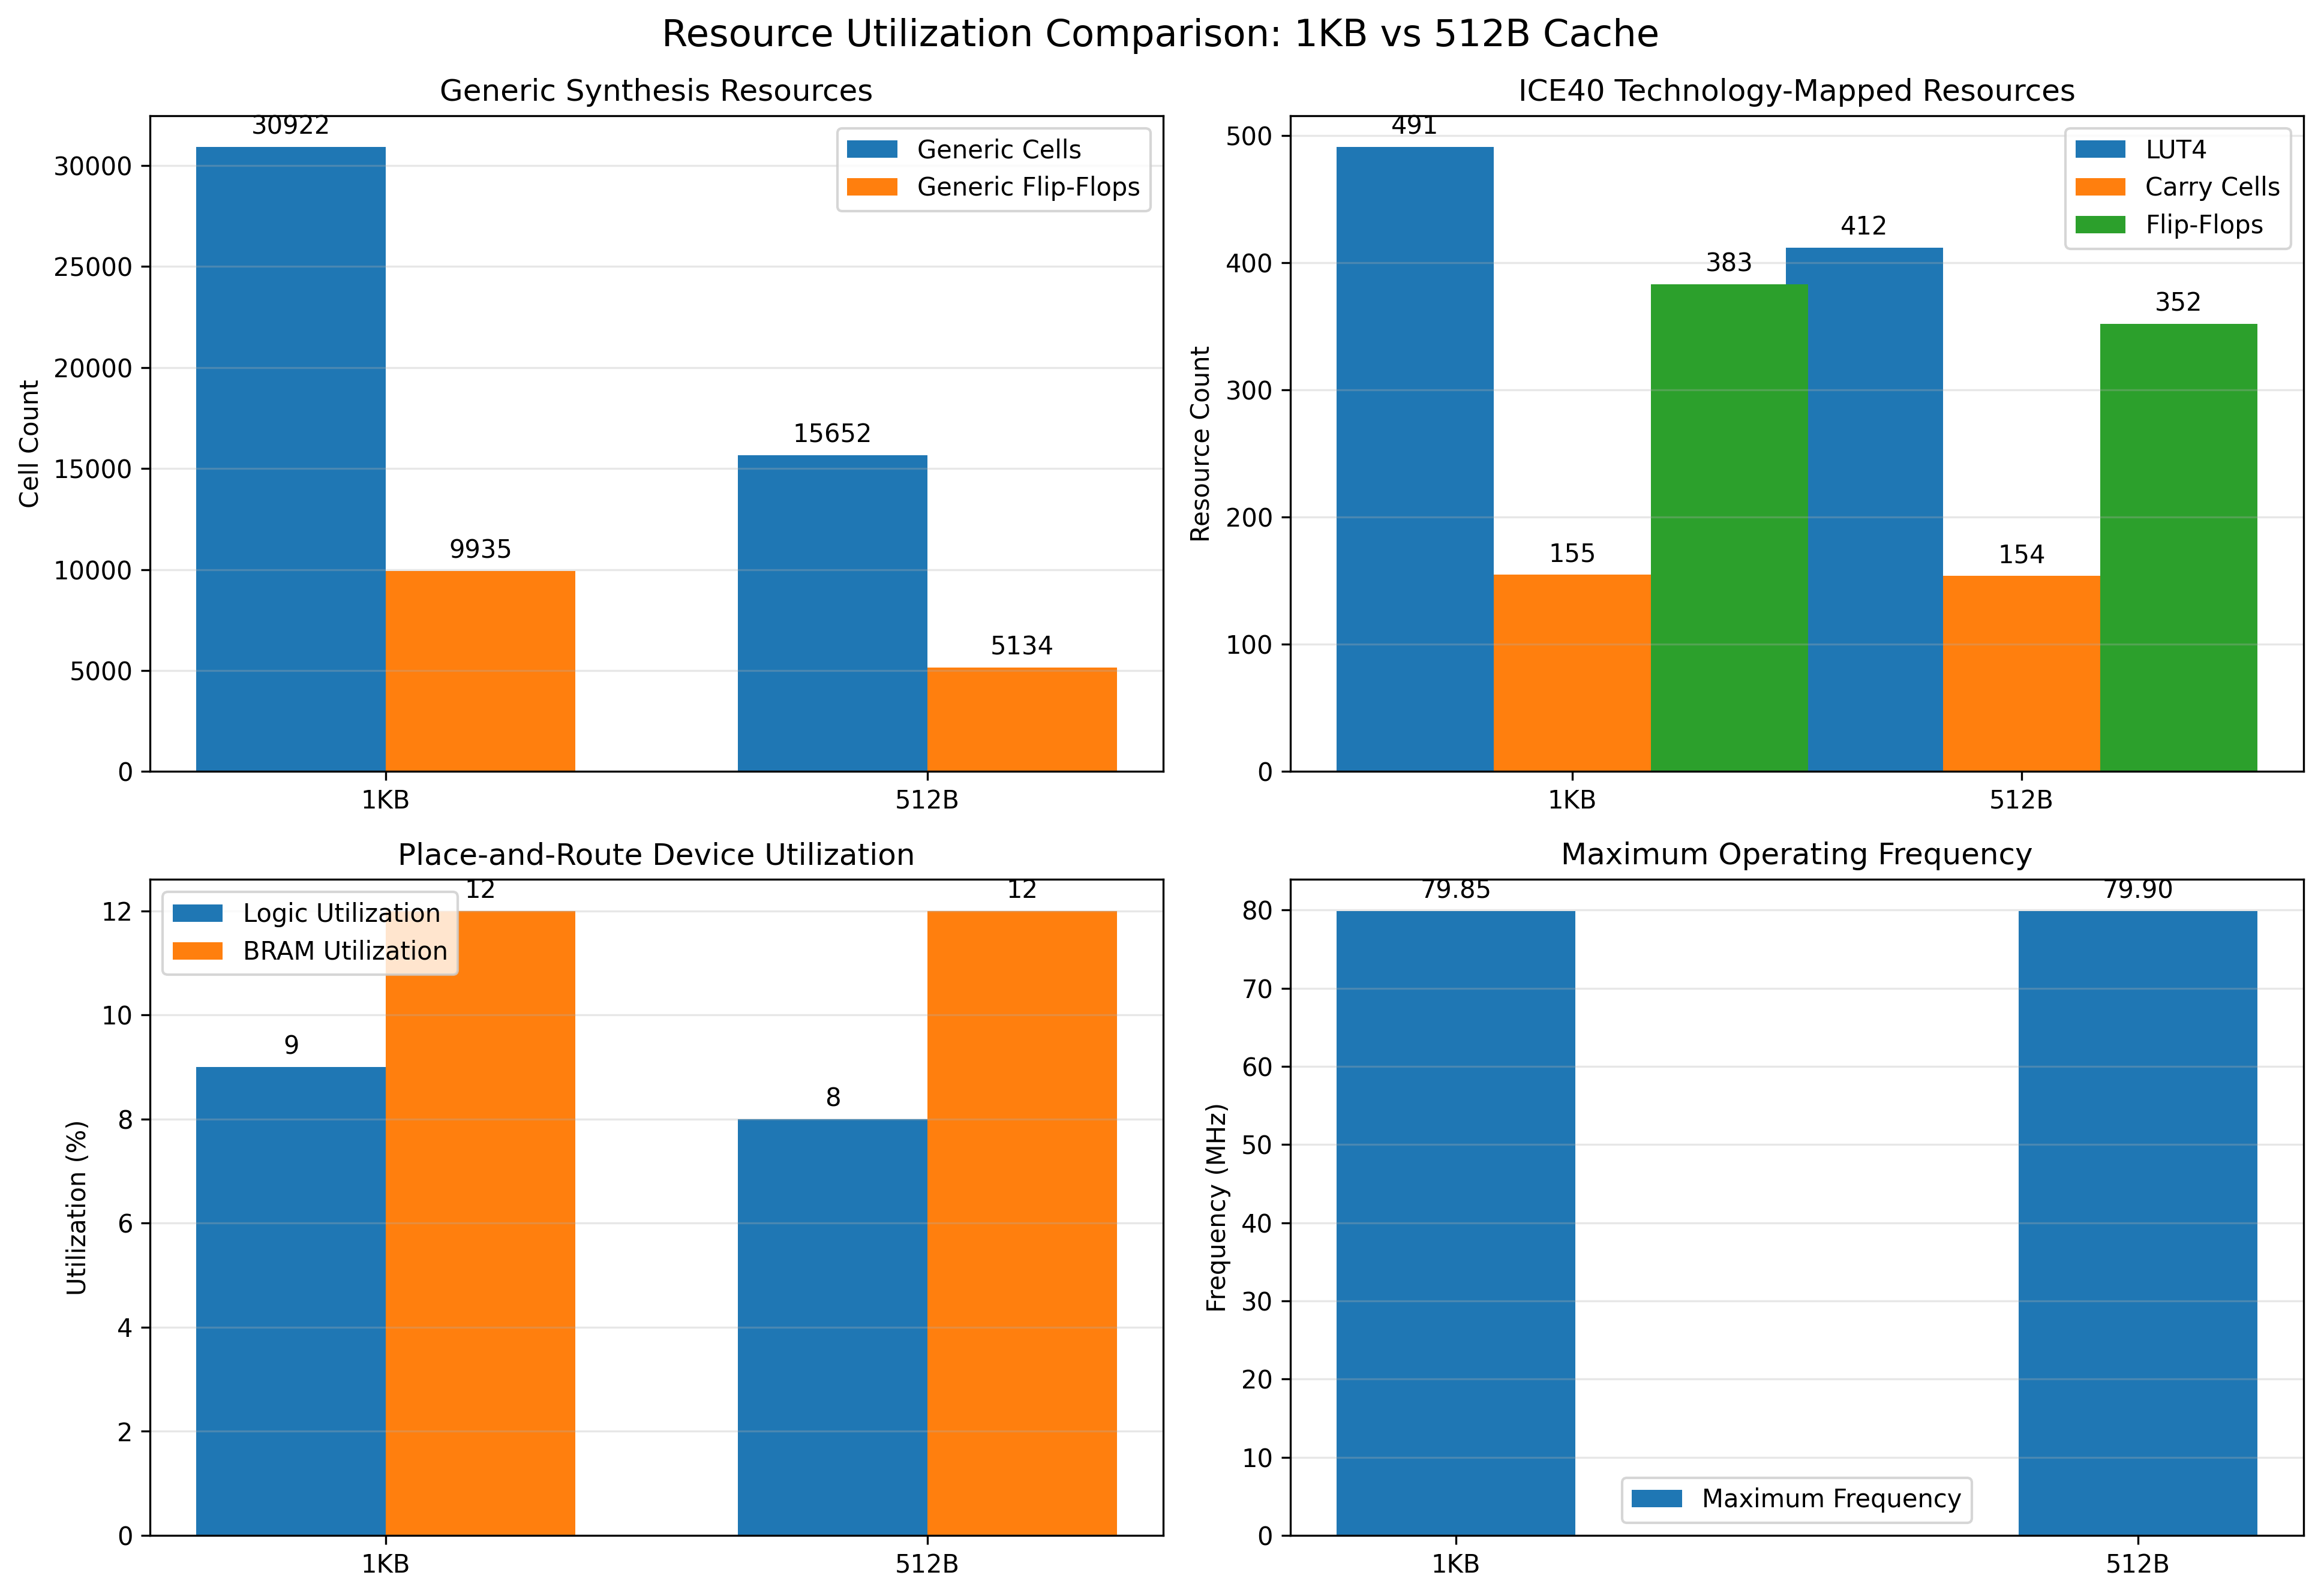
\includegraphics[width=\columnwidth]{figures/resource_comparison.png}
\caption{FPGA resource utilization comparison between 1 KB and 512 B configurations on the Lattice iCE40 HX8K FPGA.}
\label{fig:synth_res}
\end{figure}

The generic cell counts (30,922 cells, 9,935 FFs for 1~KB) represent unmapped flip-flop expansion of memory arrays and do not reflect physical FPGA cost. Technology mapping infers four embedded BRAM primitives (2 for 32-bit data RAM, 2 for 22/23-bit tag RAM). BRAM consumption is identical between 1~KB and 512~B configurations because memory count is dictated by data and tag bit-widths rather than depth. The 383 mapped flip-flops in the 1~KB design include 128 FFs dedicated to four 32-bit statistics counters (\texttt{hits}, \texttt{misses}, \texttt{mem\_reads}, \texttt{mem\_writes}), which would be omitted in a production embedded core.

Critical-path timing analysis reveals an operating frequency of 79.85~MHz ($F_{\max}$). The critical path spans 12.52~ns: BRAM clock-to-output requires 2.15~ns, seven levels of LUT4 logic require 2.47~ns, setup requires 0.10~ns, and routing interconnect contributes 7.80~ns (62.3\% of total path delay). Logic-only delay equates to a theoretical 210~MHz, demonstrating that physical routing congestion on the target FPGA dominates timing.

\textit{Takeaway:} The cache controller synthesizes into 740 logic cells (9\%) and 4 BRAMs (12\%) on an iCE40 HX8K FPGA, achieving 79.85~MHz with routing interconnect accounting for over 62\% of cycle delay.

\subsection{Verification Summary}
Hardware verification was performed using a layered methodology across six comprehensive verification activities:
\begin{enumerate}
    \item \textbf{Directed Testbench (\texttt{tb\_dm\_cache.v})}: Evaluated cold start misses, sequential reads, repeated hits, conflict thrashing, write-hit data coherence, write-miss bypass, pseudo-random reads, and full 64-line residency, completing with zero errors (\texttt{ALL TESTS PASSED}).
    \item \textbf{Write-Allocate Testbench (\texttt{tb\_write\_allocate.v})}: Validated refill-before-write sequencing (\texttt{REFILL} $\rightarrow$ \texttt{WRITEMEM} $\rightarrow$ \texttt{DONE}) on write misses, reporting \texttt{ALL WRITE-ALLOCATE TESTS PASSED}.
    \item \textbf{Memory Latency Sweeps (\texttt{tb\_lat\_sweep.v})}: Executed directed tests under $\text{LAT}\in\{2, 4, 8\}$, passing all checks.
    \item \textbf{Write Traffic and Coherence (\texttt{tb\_traffic.v})}: Executed all 9 trace files under both write policies against a reference memory array; all 18 runs reported \texttt{DATA CHECK PASSED}.
    \item \textbf{Fault-Injection Testing}: To verify testbench observability, the valid-bit check in line 47 of \texttt{rtl/dm\_cache.v} was artificially disabled. The testbench immediately flagged the initial post-reset read as invalid and captured 275 cumulative verification errors (Fig.~\ref{fig:fault}) before the condition was restored.
    \item \textbf{Gate-Level Netlist Simulation}: Post-synthesis netlists for both 1~KB and 512~B configurations were simulated with Lattice iCE40 cell models, achieving 9/9 trace passes with correct data verified against the reference memory array.
\end{enumerate}

\begin{figure}[htbp]
\centering
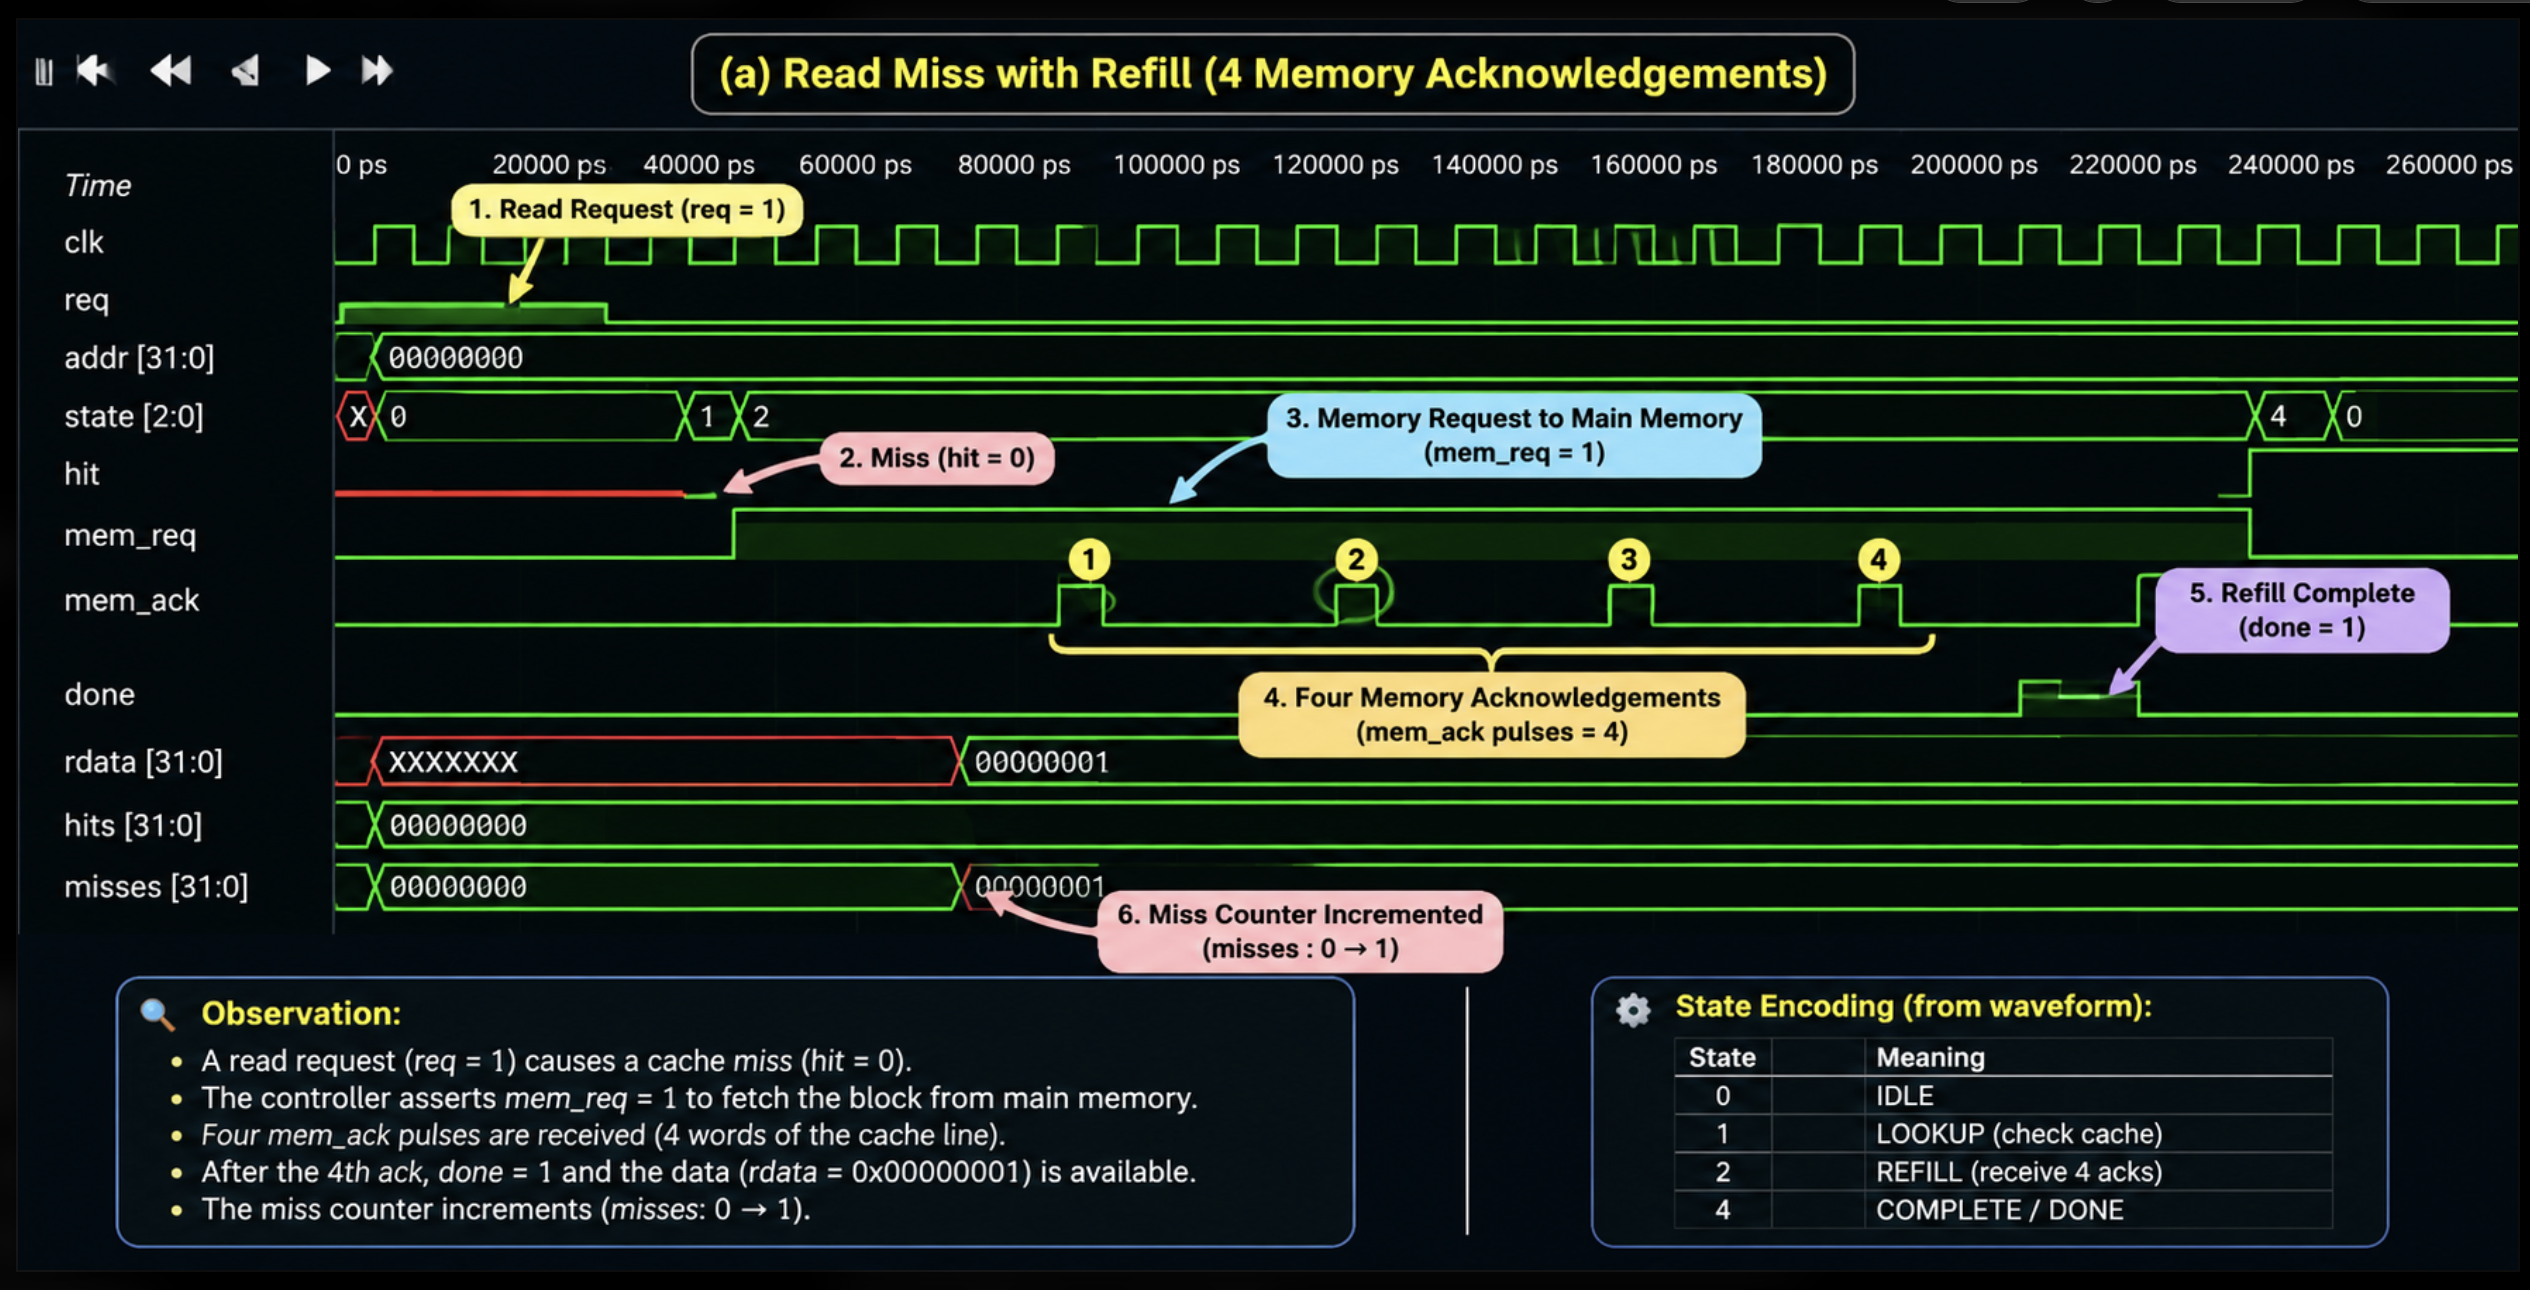
\includegraphics[width=\columnwidth]{figures/read_miss_refill.png}
\caption{Annotated waveform of a read miss and 4-word refill sequence: controller transitions IDLE $\rightarrow$ LOOKUP $\rightarrow$ REFILL $\rightarrow$ DONE, retrieving four 32-bit words with handshake.}
\label{fig:wave_refill}
\end{figure}

\begin{figure}[htbp]
\centering
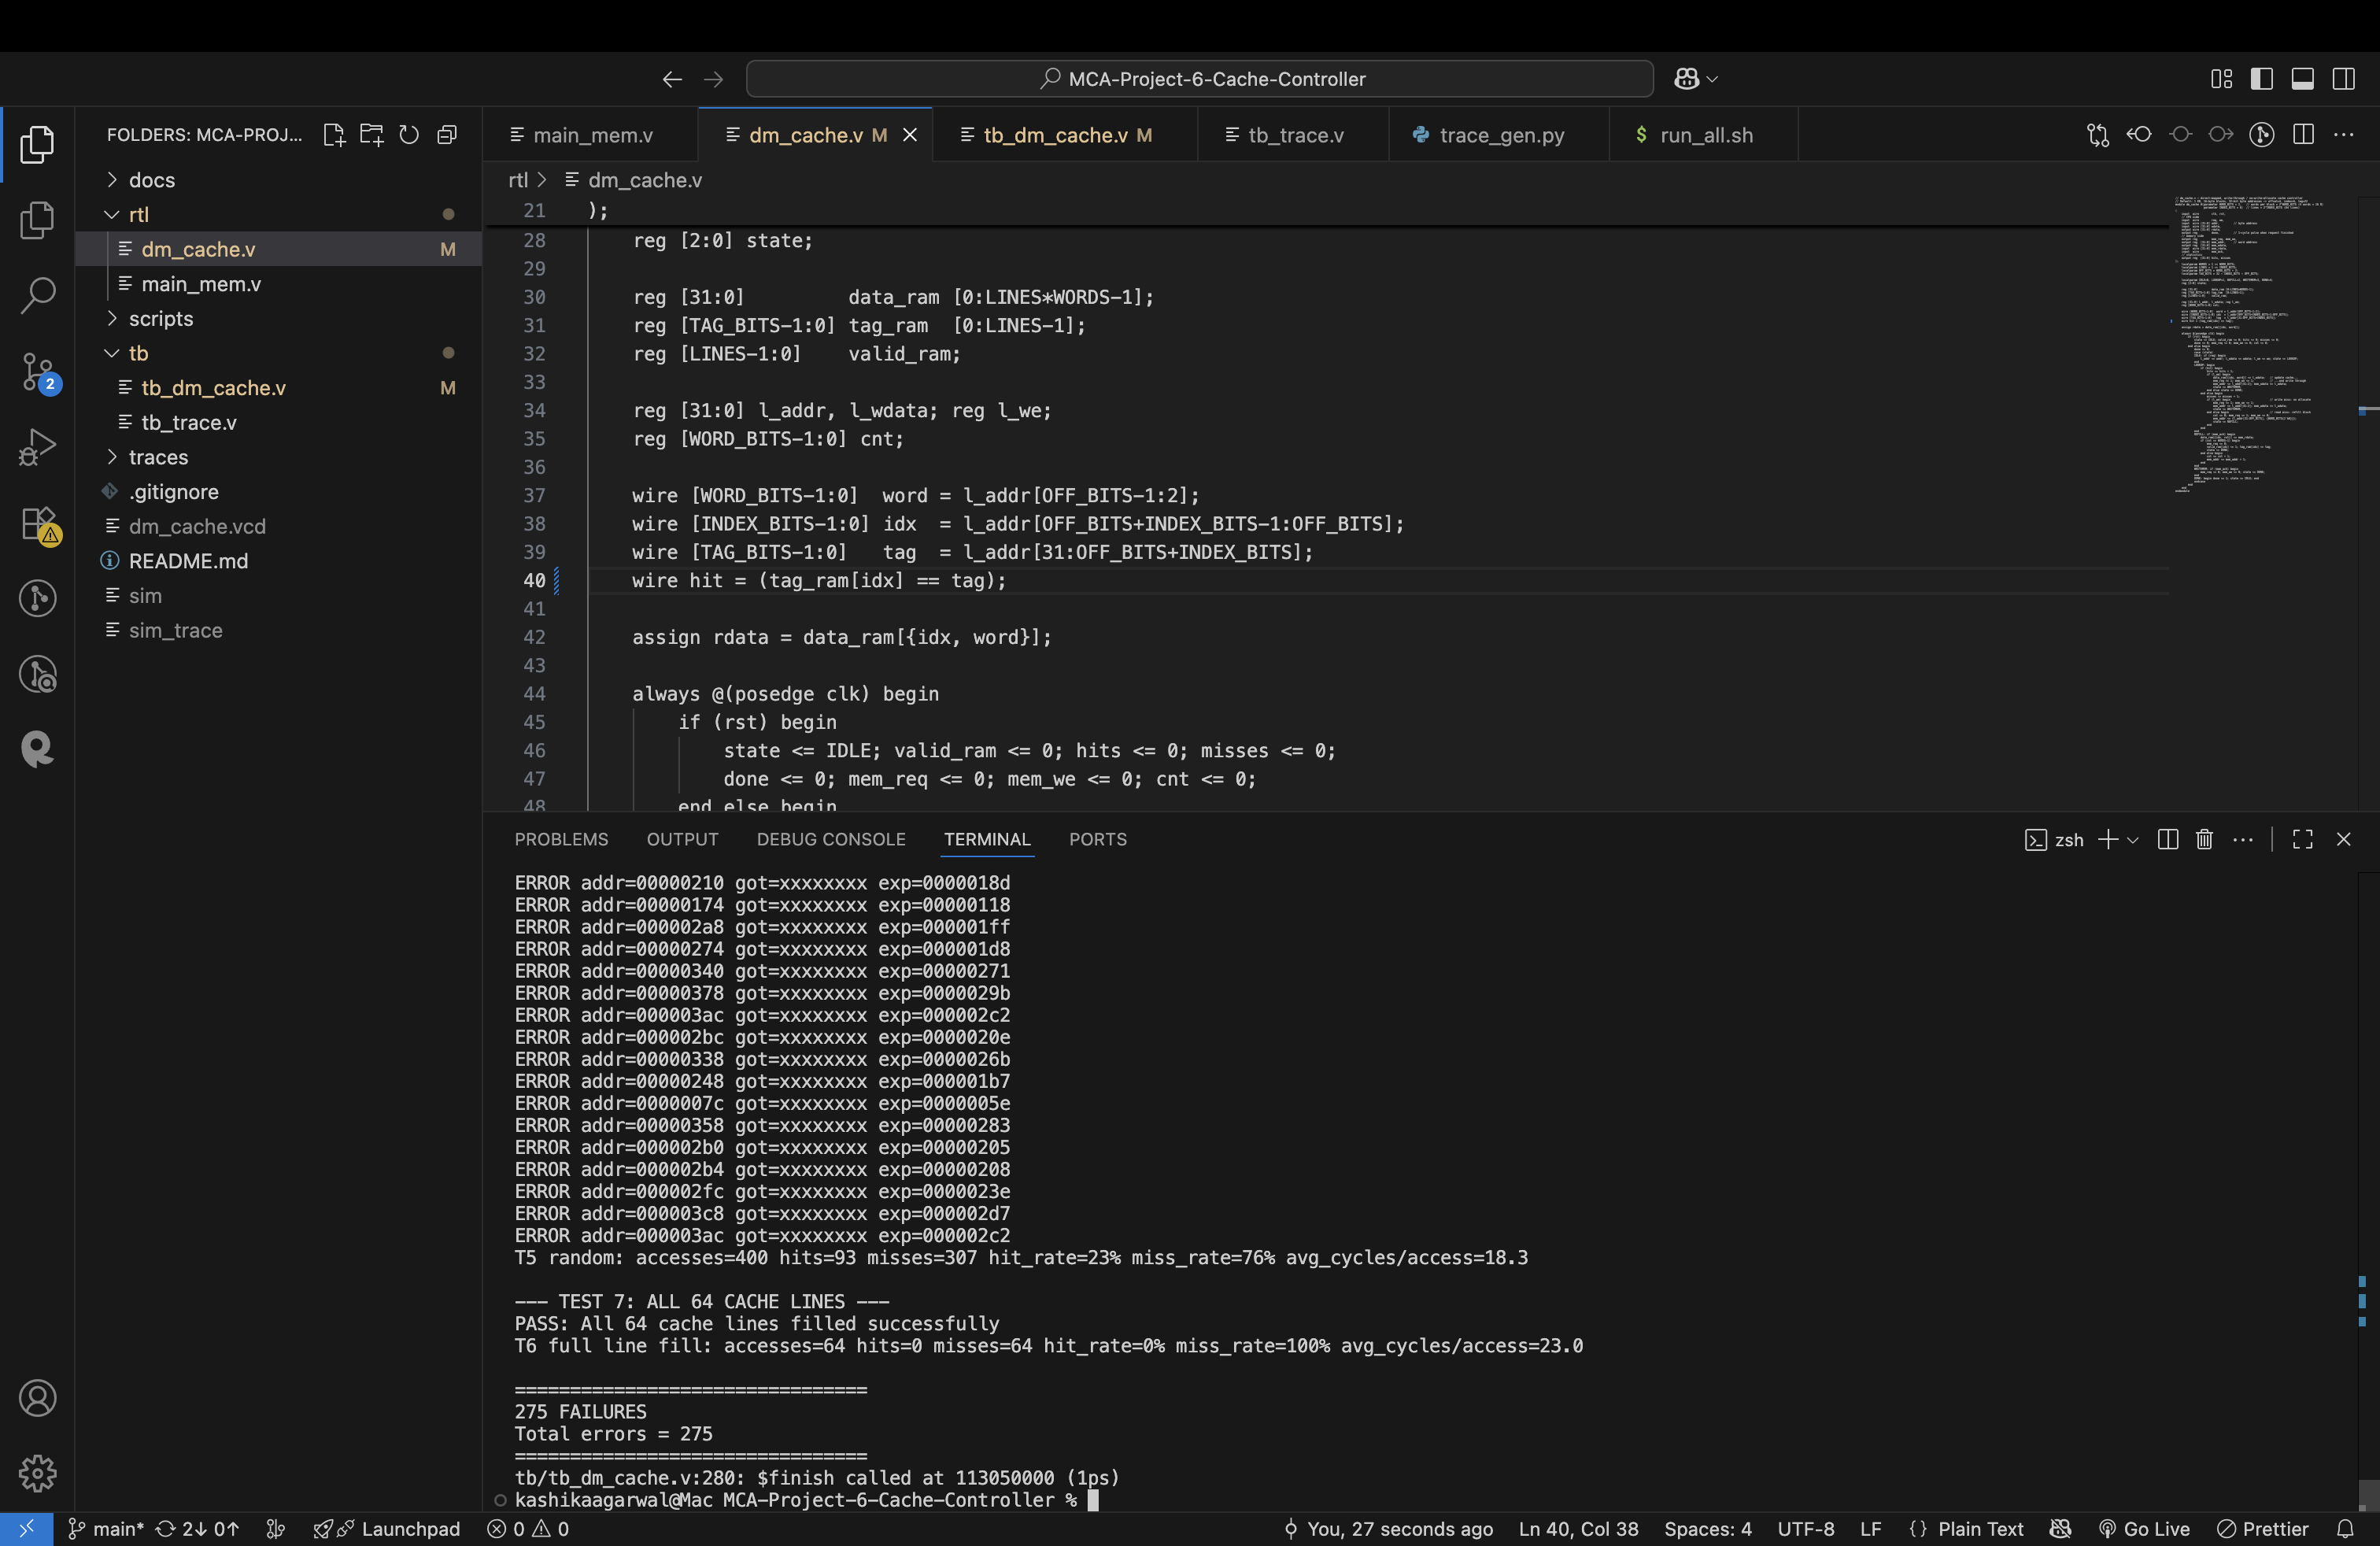
\includegraphics[width=\columnwidth]{figures/valid_check_removal_275_failures.png}
\caption{Fault-injection simulation: deliberate removal of the valid-bit check condition triggers 275 errors in the verification suite, demonstrating testbench coverage.}
\label{fig:fault}
\end{figure}

\textit{Takeaway:} Comprehensive testbench suites, gate-level simulations, and deliberate fault injection confirming 275 caught errors verify the functional correctness and robustness of the controller.

\section{Individual Contributions}
Project responsibilities and verifiable Phase II contributions for Team T109 are cataloged in Table~\ref{tab:contributions}.

% Source: README.md, docs/synthesis/synthesis.md, docs/verification_summary.md
\begin{table}[htbp]
\caption{Team T109 Individual Contributions and Phase II Ownership}
\label{tab:contributions}
\centering
\begin{tabular}{lll}
\toprule
\textbf{Name} & \textbf{Role in Phase II} & \textbf{Files / Work Owned} \\
\midrule
Priyal & Datapath \& Perf. Lead & \texttt{rtl/dm\_cache.v} datapath, parameter sweep curation \\
Anusha & Controller \& Synth. Lead & \texttt{docs/synthesis/synthesis.md}, \texttt{syn\_wrap.v}, \\
& & \texttt{scripts/run\_synth.sh}, \texttt{tb\_traffic.v}, \texttt{run\_traffic.sh} \\
Kashika & Verification Lead & \texttt{tb\_dm\_cache.v}, \texttt{tb\_write\_allocate.v}, \\
& & \texttt{tb\_lat\_sweep.v}, fault-injection, \texttt{verification\_summary.md} \\
Vaishnavi & Traces \& Plots Lead & \texttt{traces/*.trace}, \texttt{scripts/trace\_gen.py}, \\
& & Plot generation scripts (\texttt{plot\_*.py}), \texttt{docs/results/plots/} \\
Sarthak & Report \& Demo Lead & IEEE technical report (\texttt{report/Source/}), PDF generation, \\
& & \texttt{viva\_prep.md}, results integration, demo preparation \\
\bottomrule
\end{tabular}
\end{table}

\section{Conclusion}
Experimental evaluation of the 1~KB direct-mapped cache controller demonstrates a 75.00\% hit rate and 8.00-cycle AMAT on sequential access, reaching 99.50\% hit rate and 3.10-cycle AMAT under high temporal locality. Investigation of write policies establishes that while write-allocate enhances hit rate from 71.05\% to 84.21\% on write-and-read-back sequences, it doubles bus traffic on streaming writes from 512 to 1024 words. On the Lattice iCE40 HX8K FPGA, the design achieves 79.85~MHz post-routing frequency while occupying only 740 logic cells (9\%) and 4 block RAMs (12\%), with post-synthesis gate-level simulations confirming 9/9 trace passes with correct functional data.

The current implementation has three primary design limitations: (1) the controller is non-pipelined and blocking, handling only a single CPU request at a time; (2) the memory interface relies on a fixed-latency model without multi-word burst transfer capabilities, preventing spatial prefetching advantages from being realized in cycle counts; and (3) the baseline write policy is write-through with no-write-allocate, requiring off-chip memory transactions on every store operation unless the optional \texttt{WRITE\_ALLOCATE} mode is enabled.

Future architectural enhancements for Phase III include implementing a non-blocking controller with hit-under-miss capability to support pipelined processors, designing a burst-mode SDRAM/DDR interface to exploit memory row buffers, incorporating a write-back policy with dirty bits to eliminate redundant write traffic, and implementing 2-way and 4-way set associativity with pseudo-LRU replacement to resolve the conflict misses observed in column-major and large-stride workloads.

\begin{thebibliography}{00}
\bibitem{hennessy_patterson} J. L. Hennessy and D. A. Patterson, \textit{Computer Architecture: A Quantitative Approach}, 6th ed. Cambridge, MA: Morgan Kaufmann, 2017.
\bibitem{patterson_hennessy} D. A. Patterson and J. L. Hennessy, \textit{Computer Organization and Design: The Hardware/Software Interface}, 5th ed. Waltham, MA: Morgan Kaufmann, 2014.
\bibitem{smith_cache} A. J. Smith, ``Cache Memories,'' \textit{ACM Computing Surveys}, vol. 14, no. 3, pp. 473--530, Sep. 1982.
\bibitem{jouppi_pref} N. P. Jouppi, ``Improving direct-mapped cache performance by the addition of a small fully-associative cache and prefetch buffers,'' in \textit{Proc. 17th Annu. Int. Symp. Comput. Archit. (ISCA)}, 1990, pp. 364--373.
\bibitem{yosys} C. Wolf, ``Yosys Open SYnthesis Suite,'' 2016. [Online]. Available: \url{https://yosyshq.net/yosys/}
\bibitem{nextpnr} D. Shah, E. Hung, C. Wolf, S. Bazanski, D. Gisselquist, and M. Milanovic, ``nextpnr: a portable framework for FPGA place and route,'' in \textit{Proc. IEEE 27th Annu. Int. Symp. Field-Program. Custom Comput. Mach. (FCCM)}, 2019, pp. 1--4.
\bibitem{ice40} Lattice Semiconductor, ``iCE40 LP/HX Family Data Sheet,'' FPGA-DS-02029 (formerly DS1040), Rev.~3.5, Sep.~2018.
\end{thebibliography}

\end{document}
